\setcounter{chapter}{20}

\chapter{Designing Effective Graphs}\label{c21:ChapGraphs}

{\small \textit{Chapter Preview}.\footnote{This chapter is based on
``Designing Effective Graphs,'' by Edward W. Frees and Robert B.
Miller, 1990, \textit{North American Actuarial Journal}, volume 2,
number 2, 53-70. Published by the Society of Actuaries - reprinted
with permission.} Actuaries, like other business professionals,
communicate quantitative ideas graphically. Because the process of
reading, or decoding, graphs is more complex than reading text,
graphs are vulnerable to abuse. To underscore this vulnerability, we
give several examples of commonly encountered graphs that mislead
and hide information. To help creators design more effective graphs
and to help viewers recognize misleading graphs, this chapter
summarizes guidelines for designing graphs that show important
numerical information. When designing graphs, creators should:

(1) Avoid chartjunk

(2) Use small multiples to promote comparisons and assess change

(3) Use complex graphs to portray complex patterns

(4) Relate graph size to information content

(5) Use graphical forms that promote comparisons

(6) Integrate graphs and text

(7) Demonstrate an important message

(8) Know the audience.

Some of these guidelines for designing effective graphs, such as
(6), (7) and (8), are drawn directly from principles for effective
writing. Others, such as guidelines (3), (4) and (5), come from
cognitive psychology, the science of perception. Guidelines (1) and
(2) have roots both in effective writing and in graphical
perception. For example, the writing principle of brevity
demonstrates how eliminating pseudo three-dimensional perspectives
and other forms of chartjunk improve graphs. As another example, the
writing principle of parallel structure suggests using small
multiple variations of a basic graphical form to visualize complex
relationships across different groups and over time.


To underscore the scientific aspect of graphical perception, we
examine the process of communicating with a graph, beginning with a
sender's interpretation of data and ending with a receiver's
interpretation of the graph. In keeping with scientific tradition,
this chapter discusses several studies in the literature on the
effectiveness of graphs.

We conclude that the actuarial profession has many opportunities to
improve its practice, making communication more efficient and
precise.}


\section{Introduction}\label{S21:Intro}

Like other business professionals, actuaries communicate ideas
orally and in writing, as well as through presentations, which are
interactive forms of communication that encompass oral and written
messages. Actuaries, as well as other financial analysts,
communicate ideas with important quantitative components. Writers
express quantitative ideas as (1) numbers within paragraphs, (2)
numbers within tabular forms, (3) functional relationships such as
equations, and (4) data or equations as graphs.

Graphs are a simple yet powerful medium for written communication of
quantitative ideas. Graphs can present a large amount of data in a
small space, express important relationships between quantities,
compare different sets of data, and describe data, thus providing a
coherent picture of complex systems. Graphs do more than merely
state an idea; they demonstrate it.

Graphs are powerful because they are flexible, but flexibility can
be a disadvantage because of the potential for abuse. Well-accepted
references dealing with methods of quantitative data presentation
mitigate opportunities for abuse. The \emph{Chicago Manual of Style}
(1993), a standard reference, discusses presentation of in-text
data, and Ehrenberg (1977) and Tufte (1983) discuss presentation of
tabular data. In contrast, we focus on data presentation through
\emph{graphical} displays.

This chapter seeks to improve actuarial practice as it relates to
graphical displays. We intend to: (1) demonstrate the importance of
graphical displays, (2) provide guidelines to improve graphical
practice, and (3) introduce some of the scientific underpinnings of
good graphical practice. The agenda is ambitious, yet the goal of
this chapter is to provide practicing actuaries with basic tools
that they can use to become critical consumers and effective
producers of graphs. We also hope that readers will adopt our
enthusiasm and wish to explore the graphical design literature on
their own.

An important theme of this chapter is that principles of vigorous
writing can and should be applied to the practice of making
effective graphs. The \emph{Elements of Style} (Strunk and White
1979, p. xiv) summarizes vigorous writing:

\marginparjed{``\ldots sixty-three words that could change the
world.''}

\smallskip \boxedjed

Vigorous writing is concise. A sentence should contain no
unnecessary words, a paragraph no unnecessary sentences, for the
same reason that a drawing should have no unnecessary lines and a
machine no unnecessary parts. This requires not that the writer make
all his sentences short, or that he avoid all detail and treat his
subjects only in outline, but that every word tell.

\end{boxedminipage}

\smallskip

White attributes this quotation to William Strunk. White calls it
``a short, valuable essay on the nature and beauty of
brevity--sixty-three words that could change the world.'' We argue
that brevity is especially important when making effective graphs.
This was also understood by Strunk; as noted above, he said ``a
drawing should contain no unnecessary lines \ldots'' We use the term
\emph{chartjunk}, introduced by Tufte (1983), for any unnecessary
appendage in a graph.\index{plots!chartjunk}


\marginparjed{Chartjunk is any unnecessary appendage in a graph.}

Vigorous writing principles other than brevity also apply to the
practice of making effective graphs. Just as with writing, effective
graphs are the result of repeated revising and editing. Poorly
designed graphs can and do hide information and mislead. Fancy or
pretentious graphs are distracting when simpler graphs suffice.


Although the principles of effective writing are valuable, they are
not sufficient for producing effective graphs. Writing is processed
in a serial manner, word by word, sentence by sentence, with a
beginning and an ending. The process of ``reading,'' or
\emph{decoding}, a graph is nonlinear and more complex. The
additional complexities mean that even authors who follow effective
writing practices may produce ineffective graphs. Often the form of
written prose is the sole determinant of its value, whereas in
graphics the communication process plays the dominant role. We
assume that readers are familiar with effective writing forms. Thus,
we first review the communication process in which a graph plays a
crucial role.

To underscore the importance of effective graphical design, Section
\ref{S21:GDesign} provides several illustrations of graphs that hide
information and are misleading; the defects illustrated are more
serious drawbacks than mere chartjunk. The Section \ref{S21:GDesign}
illustrations motivate the need for additional guidelines and
methods for constructing effective graphs.

Section \ref{S21:DesignGuide} introduces eight important guidelines
for creating and viewing graphs. Although the guidelines do not
provide a panacea for all graphical defects, they do provide
business professionals such as actuaries with a key checklist for
creating effective graphs. The guidelines are organized so that the
first two, on chartjunk and the use of multiples, are based on both
effective writing and graphical perception perspectives. Guidelines
Three, Four and Five are related primarily to the graphical
perception literature, whereas Guidelines Six, Seven and Eight are
based primarily on effective writing principles.

As with effective writing, questions of style enter into the
discussion of what is and what is not an effective graph. Many style
decisions are based upon accepted practices without a firm
scientific foundation. However, the process of perceiving graphs has
been the subject of inquiry in several scientific disciplines,
including psychophysics, cognitive psychology, and computational
visions (Cleveland 1995, Chapter 4). Section
\ref{S21:EmpiricalFoundations} illustrates some types of
experimental evidence for determining an effective graphical form
based on both the receiver and the graph itself as units of study.
Section \ref{S21:EmpiricalFoundations} also illustrates how such
mainstays of business publications as bar charts and pie charts are
poor communicators of numerical information.

Sections \ref{S21:Conclude} and {S21:References} contain concluding
remarks and descriptions of some resources for actuaries who wish to
learn more about designing effective graphs.

Most readers are removed from the detailed data summarized by a
graph. Several difficulties and misconceptions can arise owing to
the distance between the original data and a viewer's interpretation
of the graph. Figure \ref{F21:Flowchart} illustrates the challenge
of communicating with a graph. The sender (and creator) of the graph
has a message derived from an interpretation of data. Although a few
graphs communicate raw data, the primary purpose of most graphs is
to communicate the sender's interpretation. The message the sender
intends is encoded in a graph and passed on to the receiver.

\begin{figure}[htp]
  \begin{center}
    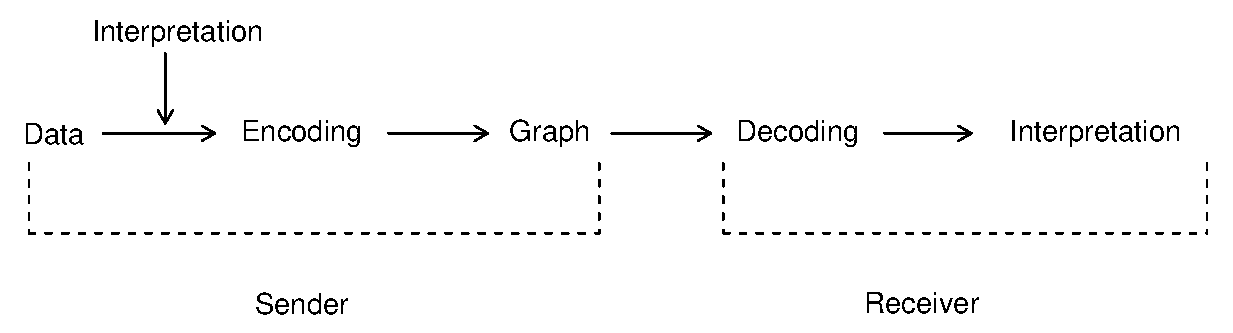
\includegraphics[width=.8\textwidth]
        {Chapter21Graphs/Fig21_1FlowChart.eps}
    \caption{\label{F21:Flowchart} \small Flow Chart of the Process of
Communicating with a Graph. The graph is a crucial intermediary in
the process of communicating data interpretation to the receiver.}
  \end{center}
\end{figure}

In general, the receiver is party to neither the exact
interpretation intended by the sender nor the raw data. Thus the
receiver must decode the graph and develop an interpretation of its
message. Two issues arise:
\begin{itemize}
\item Whether the interpretation constructed
by the receiver is congruent to the interpretation of the sender

\item Whether the receiver's
interpretation is consistent with and supported by the data.

\end{itemize}

The first issue depends on the skill with which the sender
constructs the graph and the skill with which the receiver decodes
it. A poorly constructed graph can hide or distort the sender's
message. A graph that is hard to read can discourage the receiver
from spending the time necessary to decode the message correctly.
The receiver can ignore or misinterpret a graph that is not
constructed with care.

The second issue depends not only on the skills mentioned above but
also on the skill with which the sender draws meaning from the data.
How carefully does the sender document the process of
interpretation? Is this communicated to the receiver? Is the
receiver capable of assessing the extent to which the graph is a
credible summary of the data? Failure at any of these points could
result in the receiver ignoring or misinterpreting the graph.

This chapter assumes that the graphs included in business
communications are the subject of scrutiny by serious readers.
Graphs that appear quickly on the television screen, a flip chart or
presentation package are designed to attract attention and to
entertain the viewer. Design, rather than information,
considerations dominate these media. We focus instead on graphs that
are part of professional writing and are designed to inform. As with
effective writing, we assume that in creating graphs ``\ldots one
must believe - in the truth and worth of the scrawl, in the ability
of the reader to receive and decode the message'' (Strunk and White
1979, p. 84). We now turn to examples of graphs that mislead.

\section{Graphic Design Choices Make a Difference}\label{S21:GDesign}

As noted by Schmid (1992), the ancient proverb ``One picture is
worth ten thousand words,'' when applied to graphs might well read,
``One picture \emph{can be} worth ten thousand words \emph{or
figures}.'' Graphic potential is not easily realized. Because of
their flexibility, graphs too easily render visual displays of
quantitative information that are uninformative, confusing or even
misleading.

Examples \ref{S21:GDesign}.1 through \ref{S21:GDesign}.5 illustrate
five different types of deceptive graphs. In each case, the data
were not altered nor were different dimensions of the data
portrayed. The common theme of the examples is that, by altering
only the data scales, the creator can alter dramatically a viewer's
interpretation.

\linejed

\textbf{Example \ref{S21:GDesign}.1: Including Zero To Compress
Data}. Figure \ref{F21:InsurEmploy} shows a time series of the
percentage of full-time equivalent workers employed in the insurance
industry. The annual data, 1948-1993, are from the National Income
and Product Accounts produced by the Bureau of Labor Statistics. The
left-hand panel, Figure \ref{F21:InsurEmploy}(a), provides the
impression of a stable employment environment for the insurance
industry. Including zero on the vertical axis produces this seeming
stability. By doing this, most of the graph is devoted to white
space that does not show the variability in the data. In contrast,
the right-hand panel, Figure \ref{F21:InsurEmploy}(b), uses the data
to set the range on the axes. This panel clearly shows the large
employment increases in the years following the Korean War, circa
1952. It also allows the reader to see the employment declines that
the insurance industry has suffered in the most recent three years.

\begin{figure}[htp]
  \begin{center}\subfloat[\textbf{A stable insurance
industry}]{
   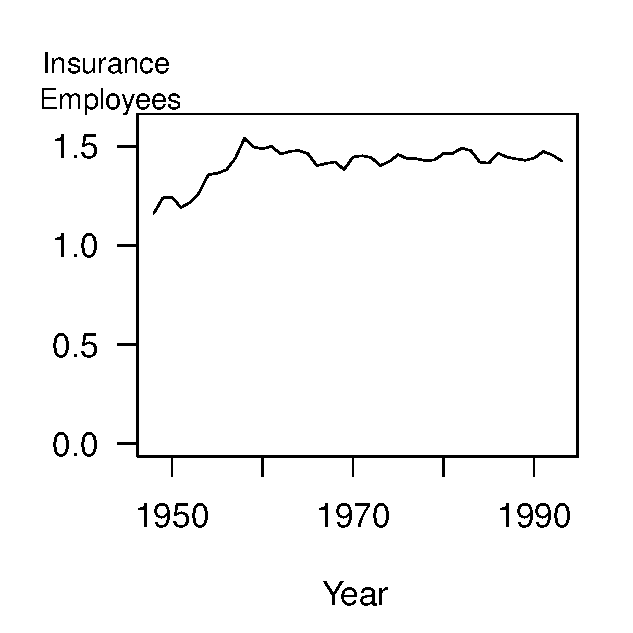
\includegraphics[width=0.45\textwidth]
   {Chapter21Graphs/Fig21_2InsurEmploya.eps}}  \hfill
   \subfloat[\textbf{The insurance industry work force increased
dramatically in the 1950s}]{
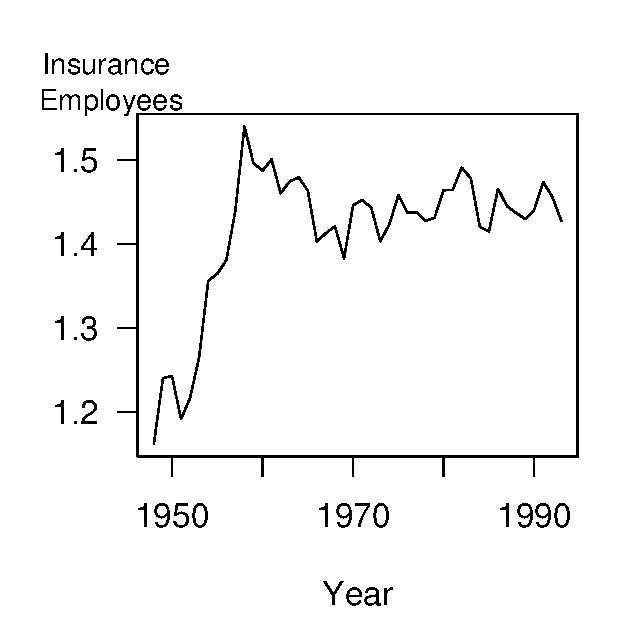
\includegraphics[width=0.45\textwidth]
        {Chapter21Graphs/Fig21_2InsurEmployb.eps}}
    \caption{\label{F21:InsurEmploy} \small Annual Insurance Employees, 1948-1993. ``Insurance employees'' is
the percentage of full-time-equivalent employees who are working for
insurance carriers. Allowing the data to determine the scale ranges
reveals interesting aspects of the data.}
  \end{center}
\end{figure}

This example is similar to a popular illustration from Huff's
well-known \emph{How to Lie with Statistics} (Huff 1954). The point
is that motivation external to the data, such as including zero on
an axis, can invite us to alter the data scale and change a viewer's
interpretation of the data. As Example \ref{S21:GDesign}.2 shows,
creators of graphs can also alter a viewer's interpretation by
changing both scales of a two-dimensional graph.

\empexjed{RiskSurvey}\index{datasets!risk managers cost
effectiveness}

\linejed

\textbf{Example \ref{S21:GDesign}.2: Perception of Correlation}.
Figure \ref{F21:FirmRMcostvsSize} relates risk management cost
effectiveness to firm size. These data are from a survey of 73 risk
managers of large, U.S.-based, international firms that was
originally reported in Schmit and Roth (1990). The data are analyzed
in Section 6.5. Here, the measure of risk management cost
effectiveness, firm cost, is defined to be the logarithm of the
firm's total property and casualty premiums and uninsured losses as
a percentage of total assets. The firm size measure is total assets
in logarithmic units.


\begin{figure}[htp]
  \begin{center}\subfloat[\textbf{The data in this figure appear
 less correlated}]{
   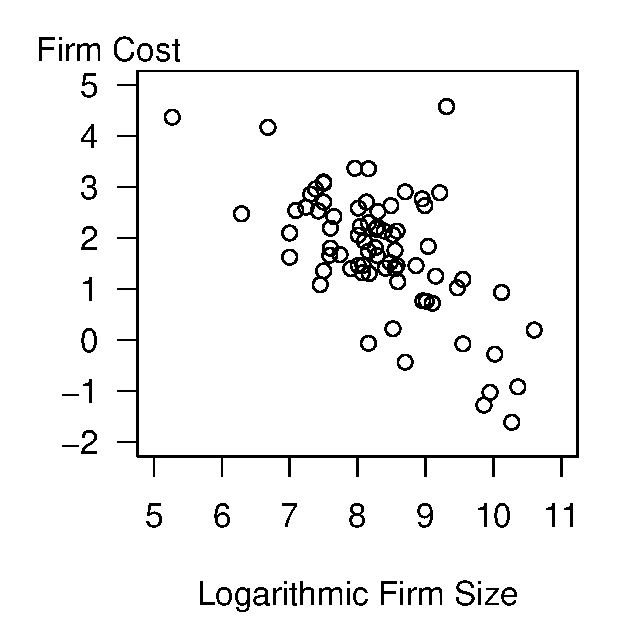
\includegraphics[width=0.45\textwidth]
   {Chapter21Graphs/Fig21_3FirmRMcostvsSizea.eps}}  \hfill
   \subfloat[\textbf{The data in this figure appear
more correlated}]{
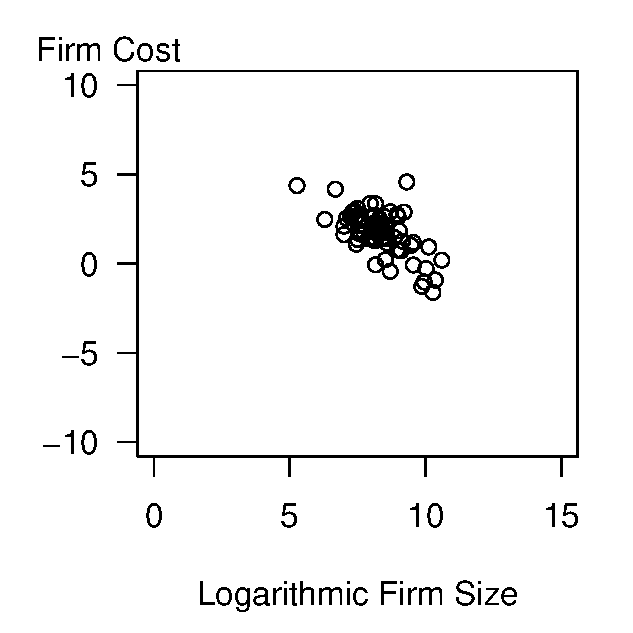
\includegraphics[width=0.45\textwidth]
        {Chapter21Graphs/Fig21_3FirmRMcostvsSizeb.eps}}
    \caption{\label{F21:FirmRMcostvsSize} \small Cost
Effectiveness of a Firm's Risk Management Practices Versus Firm
Size. The data represented in each figure are the same. However, the
wider scales in panel (b) suggest that the data are more highly
correlated.}
  \end{center}
\end{figure}


The left-hand panel, Figure \ref{F21:FirmRMcostvsSize}(a), shows a
negative relationship between firm costs and firm size, as
anticipated by Schmit and Roth. The correlation coefficient between
the two variables is -0.64. The data are in a small center portion
of Figure \ref{F21:FirmRMcostvsSize}(b) when compared to the
left-hand panel, Figure \ref{F21:FirmRMcostvsSize}(a). Figure
\ref{F21:FirmRMcostvsSize}(a) uses the data to determine the axes
and thus shows more patterns in the data. As Cleveland, Diaconis,
and McGill (1982) show, the scaling makes the data in the right-hand
panel appear more correlated than in the left-hand panel.

Change of scales can also alter the viewer's perception of trend in
time series data, as illustrated in Example \ref{S21:GDesign}.3.

\linejed

\textbf{Example \ref{S21:GDesign}.3: Transforming to a Logarithmic
Scale}. Figure \ref{F21:InsurInForce} exhibits a time series of the
U.S. credit insurance market over 1950-1989. These data are analyzed
in Frees (1996) and are originally from the \emph{Life Insurance
Fact Book} (1990). When the amount of insurance is examined on a
linear scale in Figure \ref{F21:InsurInForce}(a), the credit
insurance market appears to be expanding rapidly. However, Figure
\ref{F21:InsurInForce}(b) shows that, when examined on a logarithmic
scale, the market is leveling off. As discussed in Section 3.2.2,
changes on a logarithmic scale can be interpreted as proportional
changes. Thus, Figure \ref{F21:InsurInForce}(a) shows the market is
increasing rapidly, and Figure \ref{F21:InsurInForce}(b) shows that
the rate of increase is leveling off. These messages are not
contradictory, but viewers must interpret each graph critically to
understand the intended message.

\begin{figure}[htp]
  \begin{center}\subfloat[\textbf{U.S. credit life insurance market exploding}]{
   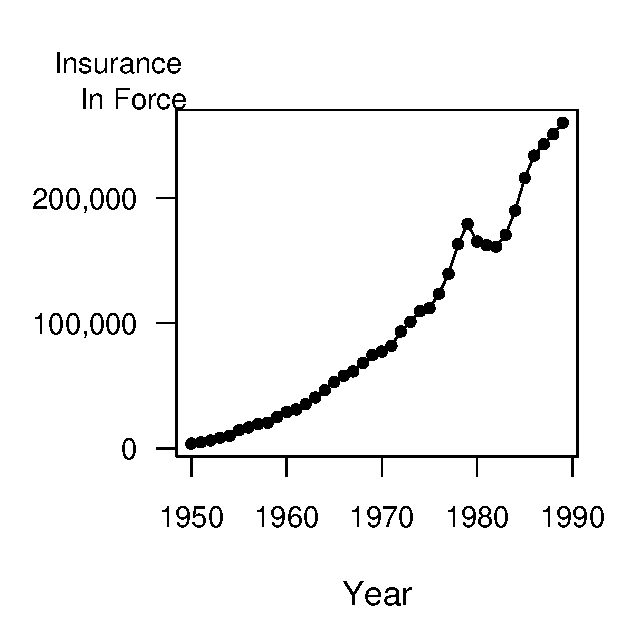
\includegraphics[width=0.45\textwidth]
   {Chapter21Graphs/Fig21_4InsurInForcea.eps}}  \hfill
   \subfloat[\textbf{U.S. credit life insurance market leveling
off}]{
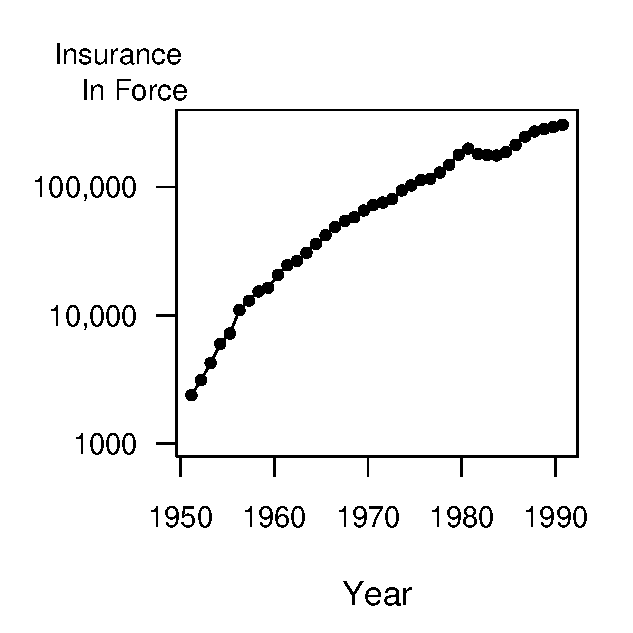
\includegraphics[width=0.45\textwidth]
        {Chapter21Graphs/Fig21_4InsurInForceb.eps}}
    \caption{\label{F21:InsurInForce} \small Annual U.S. Credit Life Insurance in Force, 1950-1989. Different
vertical scales give different impressions of the rate of growth
over time.}
  \end{center}
\end{figure}

\newpage


\linejed

\textbf{Example \ref{S21:GDesign}.4: Double Y-Axes}. Figure
\ref{F21:CPI} displays two measures of inflation that are produced
by the Bureau of Labor Statistics. On the left-hand axes are CPI\_U,
the consumer price index for urban consumers. On the right-hand axes
are CPI\_M, the consumer price index for medical components of the
overall index. Each series consists of monthly values ranging from
January 1947 through April 1995.

\begin{figure}[htp]
  \begin{center}\subfloat[\textbf{Overall Consumer Price Index (CPI) is similar to
the medical component of the CPI}]{
   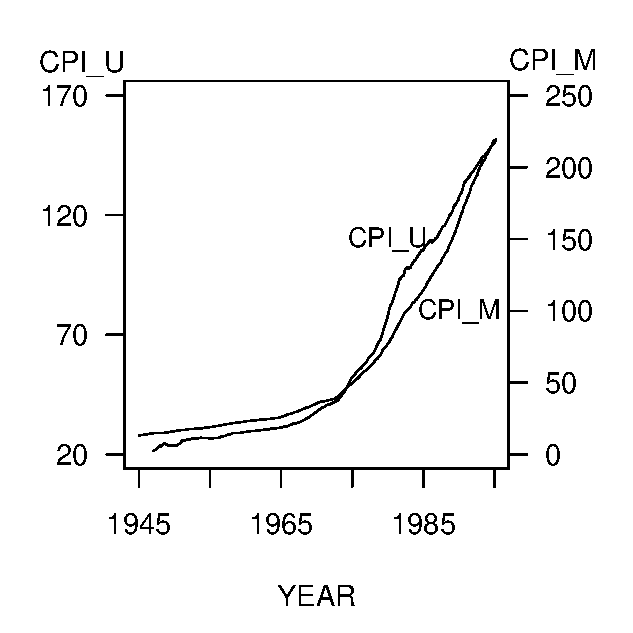
\includegraphics[width=0.45\textwidth]
   {Chapter21Graphs/Fig21_5CPIa.eps}}  \hfill
   \subfloat[\textbf{Overall Consumer Price Index
(CPI) is increasing more slowly than the medical component of the
CPI}]{
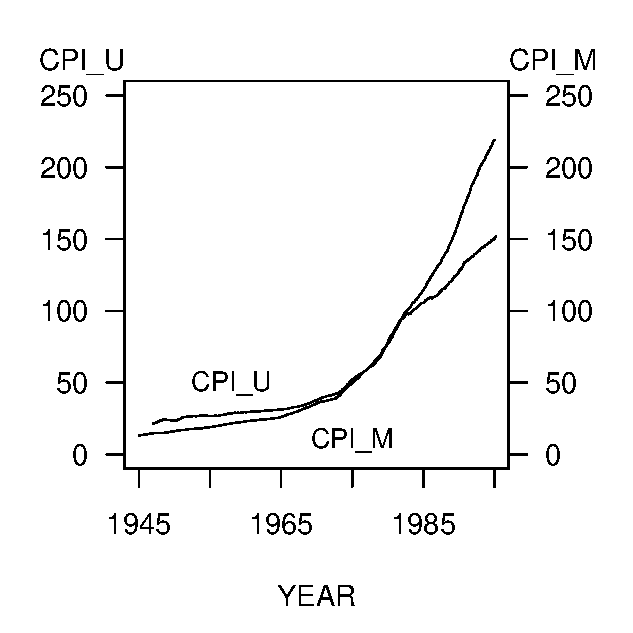
\includegraphics[width=0.45\textwidth]
        {Chapter21Graphs/Fig21_5CPIb.eps}}
    \caption{\label{F21:CPI} \small Monthly Values of the Overall Consumer Price Index (CPI) and the
Medical Component of the CPI, January 1947 through April 1995.
Different scale ranges alter the appearances of relative growth of
the two series.}
  \end{center}
\end{figure}


The left-hand panel, Figure \ref{F21:CPI}(a), suggests that the
CPI\_U and the CPI\_M begin and end in approximately the same
position, thus implying that they have increased at about the same
rate over the period. The creator could argue that each index
measures the value of a standard bundle of goods, thus justifying
the argument for using a different scale for each series.

The right-hand panel, Figure \ref{F21:CPI}(b), provides a more
useful representation of the data by using the same scale for each
series. Here, CPI\_M begins lower than CPI\_U and ends higher. That
is, the medical component index has increased more quickly than the
index of prices for urban consumers. Other patterns are also evident
in Figure \ref{F21:CPI}: each series increased at roughly the same
rate over 1979-1983 and CPI\_M increased much more quickly from 1983
to 1994 when compared to 1948-1979.

\linejed

\textbf{Example \ref{S21:GDesign}.5: Aspect Ratio}. Figure
\ref{F21:tsUnemploy} shows a time series plot of the monthly
unemployment rate, April 1953 through December 1992. The
unemployment rate is the percentage of unemployed civilian labor
force, seasonally adjusted. It is part of the Household Survey
produced by the Bureau of Labor Statistics, Department of Labor.
This series was analyzed in Frees et al. (1997). The top panel of
Figure \ref{F21:tsUnemploy} shows that the unemployment rate
averaged 5.9\% with a peak of 10.8\% in the fourth quarter of 1982
and a minimum of 2.7\% in the third quarter of 1953.

\begin{figure}[htp]
  \begin{center}
    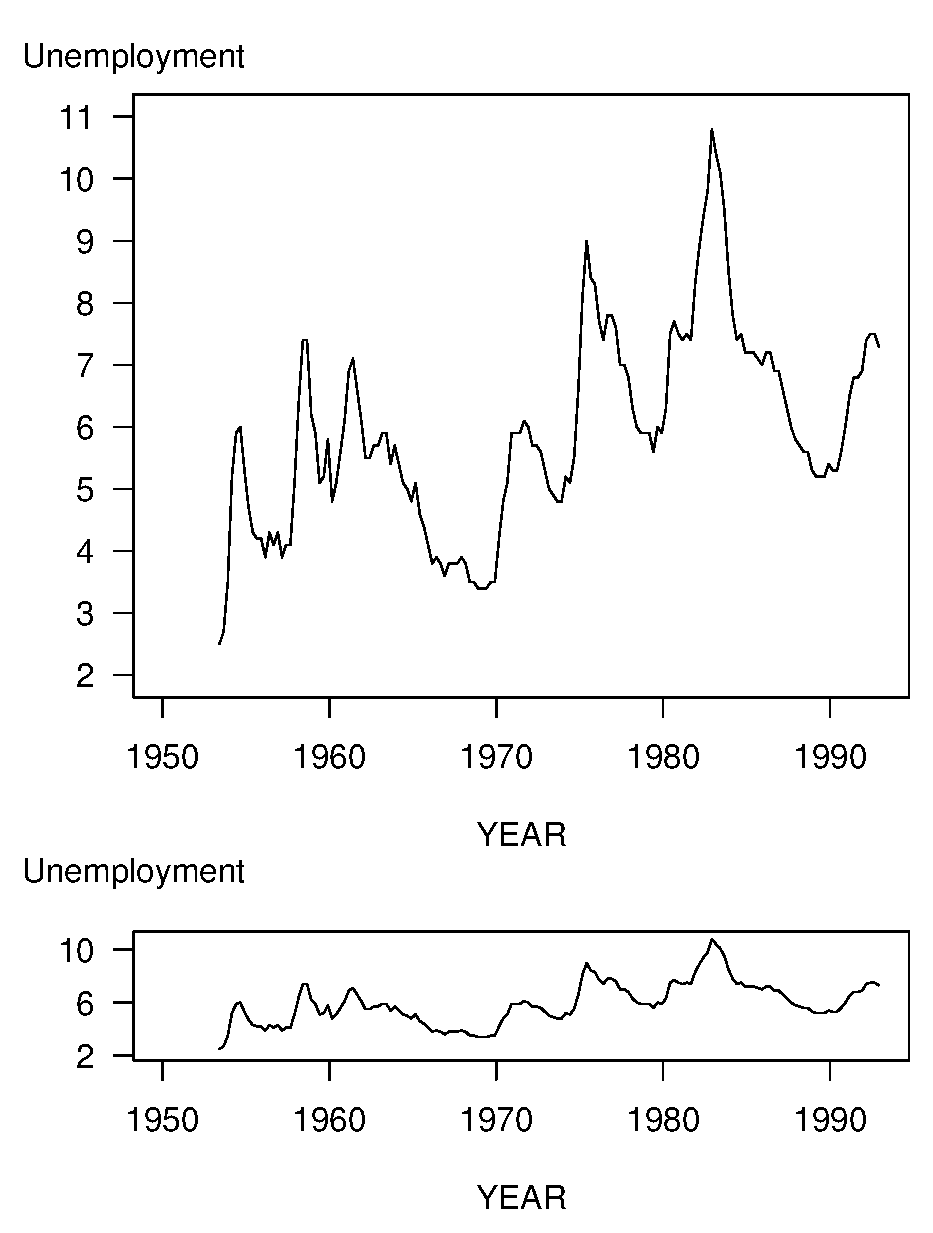
\includegraphics[width=0.45\textwidth]
        {Chapter21Graphs/Fig21_6tsUnemploy.eps}
    \caption{\label{F21:tsUnemploy} \small Time Series Plot of Quarterly Values of the U.S. Unemployment Rate,
1953-1992. The lower panel displays a feature that is not evident in
the upper panel; unemployment declines more slowly than it rises.}
  \end{center}
\end{figure}


The two panels in Figure \ref{F21:tsUnemploy} differ only in their
shape, not in the scaling of either variable or in the relative
amount of space that the data take within the figure frame. To
differentiate these two shapes, we can use the concept of a figure's
\emph{aspect ratio}, defined to be the height of the data frame
divided by its width (some sources use the reciprocal of this value
for the aspect ratio). The data frame is simply a rectangle whose
height and width just allow the graph \emph{of the data} to fit
inside. To illustrate, in the upper panel in Figure
\ref{F21:tsUnemploy}, the length of the vertical side is equal to
the length of the horizontal side. In the lower panel, the vertical
side is only 25\% of the horizontal side.

\marginparjed{A figure's aspect ratio is defined to be the height of
the data frame divided by its width.}\index{plots!aspect ratio}

Both panels show that the unemployment series oscillated widely over
this 39-year period. The lower panel, however, displays a feature
that is not apparent in the upper panel; the rise to the peak of an
unemployment cycle is steeper than the descent from the peak. Within
each unemployment cycle, the percentage of workers unemployed tends
to rise quickly to a maximum and then to fall gradually to a
minimum. This behavior is surprisingly regular over the almost
39-year period displayed in the plot.

Different aspect ratios can leave substantially different
impressions on the eye, as Figure \ref{F21:tsUnemploy} illustrates.
Thus, the aspect ratio can be chosen to emphasize different features
of the data.

\linejed

\section{Design Guidelines}\label{S21:DesignGuide}

Understanding the issues illustrated in Section \ref{S21:GDesign}
can help actuaries and other business professionals create and
interpret graphs. This section presents eight guidelines for
designing effective graphs. One of our main points is that current
practice is not in accord with these guidelines. Thus, we anticipate
that not all of our readers will find the demonstrations of the
guidelines visually appealing, but, as stated in Section
\ref{S21:Intro}, many of the guidelines are based on a scientific
foundation outlined in Section \ref{S21:EmpiricalFoundations}.
``Intuition'' is something we learn and cultivate; progress in
science does not always conform to current intuition. It was widely
believed at one time that the earth was flat and that the sun
revolved about the earth. The demonstrations of this section may or
may not be immediately intuitive, but they are logical conclusions
from the design guidelines advocated here.

\subsubsection*{Guideline One: Avoid Chartjunk}

In Section \ref{S21:Intro}, we defined chartjunk to be any
unnecessary appendage in a graph. Creators of graphs who use
chartjunk lower their credibility with serious receivers. Even when
senders convey a correct interpretation accompanied by chartjunk,
they ask receivers to process and properly ignore the chartjunk. If
chartjunk is part of the default, or easily used, options of a
software package, then the sender can clutter a graph, or even make
a graph misleading, simply by punching a button.

\marginparjed{Avoid pictures that are not worth ten thousand
words.}\index{plots!chartjunk}

Senders who avoid chartjunk raise their credibility. They ask
receivers to look only at meaningful characters and marks. Senders
may have to spend considerable time with their software to make
effective graphs, but the respect and attention of their receivers
reward them. Another way to avoid chartjunk is not to use a graph at
all if a few words will do. If the message in a graph can be
summarized in a few words, then the graph is not needed. Avoid
pictures that are not worth ten thousand words!

Avoiding chartjunk is based in part on the concept of brevity in
vigorous writing principles. From the graphical perception
viewpoint, avoiding chartjunk reduces the noise when communicating
between the graph's sender and receiver. Thus, this guideline is
important because it has roots in both writing and perception
principles.

\linejed

\textbf{Example \ref{S21:DesignGuide}.1: Premium Receipts of Life
Insurance Companies}. Figure \ref{F21:DotPlotPremiumReceipts}(a) is
an adaptation of a graph on page 69 of the \emph{Life Insurance Fact
Book }(1994). The graph reports 15 bits of information: 5 years and
2 percentages for each year (a third percentage is found by
subtraction). A three-dimensional box represents each percentage,
and each box displays different shadings to represent the three
lines of business: health, annuity and life. These figures could be
reported compactly in a small table. However, granting that a graph
may help the receiver appreciate trends in the figures, the graph's
simplicity should reflect the simplicity of the information
available in the figures. In particular, a small plotting symbol
suffices to report a percentage. A three-dimensional, shaded box is
hardly called for. It is interesting that the three-dimensional box
was an ``innovation'' in 1994. Earlier editions of the \emph{Fact
Book} used two-dimensional boxes. The volume of chartjunk took a big
jump in 1994.

\begin{figure}[htp]
  \begin{center}\subfloat[\textbf{The three-dimensional stacked bar chart
is a poor graphical form for making comparisons over time and across
lines of business}.]{
   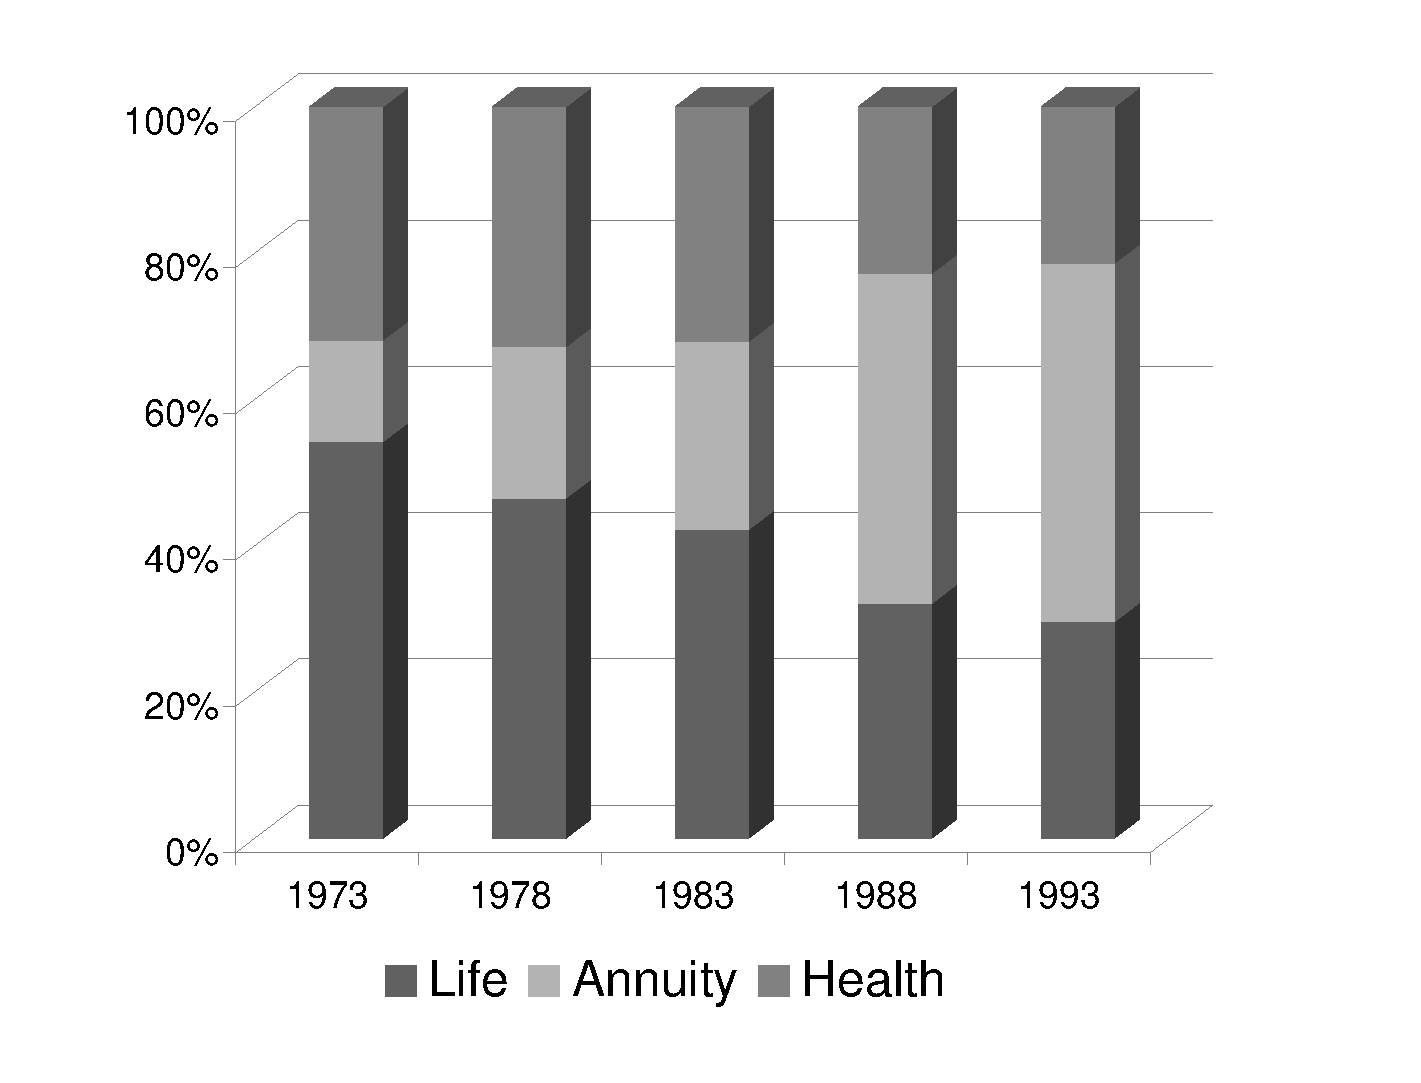
\includegraphics[width=0.45\textwidth]
   {Chapter21Graphs/3DBarChartNew.eps}}  \hfill
   \subfloat[\textbf{The dot plot allows for direct comparison over
time and across lines of business.}]{
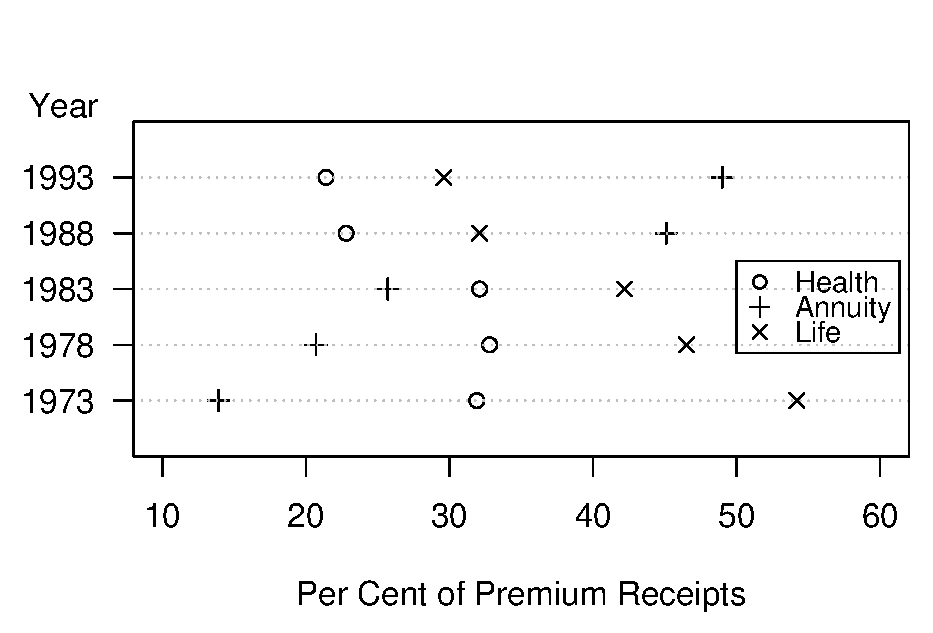
\includegraphics[width=0.45\textwidth]
        {Chapter21Graphs/Fig21_7bDotPlotPremiumReceipts.eps}}
    \caption{\label{F21:DotPlotPremiumReceipts} \small Distribution of Premium Receipts, 1973-1993. The excessive
chartjunk of (a) hides the large change in distribution types
between 1983 and 1988.}
  \end{center}
\end{figure}


Figure \ref{F21:DotPlotPremiumReceipts}(b) is a \emph{dot plot},
discussed by Cleveland (1994). Different plotting symbols show the
different lines of business. The tick marks on the lower horizontal
axes help us estimate the percentages, and the light, dotted grid
lines help us scan across the graph to the plotting symbols of
interest. The major shifts, and the approximate magnitudes of the
shifts, that happened between 1983 and 1988 are clear here.

\linejed

\subsubsection*{Guideline Two: Use Small Multiples to Promote Comparisons and Assess Change}

Statistical thinking is directed towards comparing measurements of
different entities and assessing the change of a measurement over
time or some other unit of measurement. Graphical displays are
inherently limited when portraying comparisons or assessing changes
because they are static, two-dimensional media. Graphs that contain
multiple versions of a basic graphical form, each version portraying
a variation of the basic theme, promote comparisons and assessments
of change. By repeating a basic graphical form, we promote the
process of communication.

Tufte (1997) states that using \emph{small multiples} in graphical
displays achieves the same desirable effects as using parallel
structure in writing. Parallel structure in writing is successful
because it allows readers to identify a sentence relationship only
once and then focus on the meaning of each individual sentence
element, such as a word, phrase or clause. Parallel structure helps
achieve economy of expression and draw together related ideas for
comparison and contrast. Similarly, small multiples in graphs allow
us to visualize complex relationships across different groups and
over time.

\marginparjed{Small multiples in graphs allow us to visualize
complex relationships across different groups and over time.}

The Section \ref{S21:GDesign} figures illustrated the use of small
multiples. In each figure, the two plots portrayed were identical
except for the change in scale; this use of parallel structure
allowed us to demonstrate the importance of scaling when
interpreting graphs. Example \ref{S21:DesignGuide}.2 illustrates
another application of small multiples in graphical displays,
Cleveland's (1993) multiway dot plot.

\linejed

\textbf{Example \ref{S21:DesignGuide}.2: Relative Importance of Risk
Source}. Figure \ref{F21:MultipleDotPlots}, called a \emph{multiway
dot plot}, demonstrates conclusions reached by using a model
introduced in Frees (1998) concerning the relative importance of
risk sources within a block of short-term insurance contracts. The
risk sources are the stochastic interest environment, the frequency
of claims (mortality), and the possibility of a catastrophic event
(disaster) occurring. The relative importance of these three risk
sources is considered by letting two parameters of interest vary.
These parameters are the expected year until disaster and, in the
event of disaster, the expected proportion (probability) of
policyholders that will succumb to disaster.

\begin{figure}[htp]
  \begin{center}
    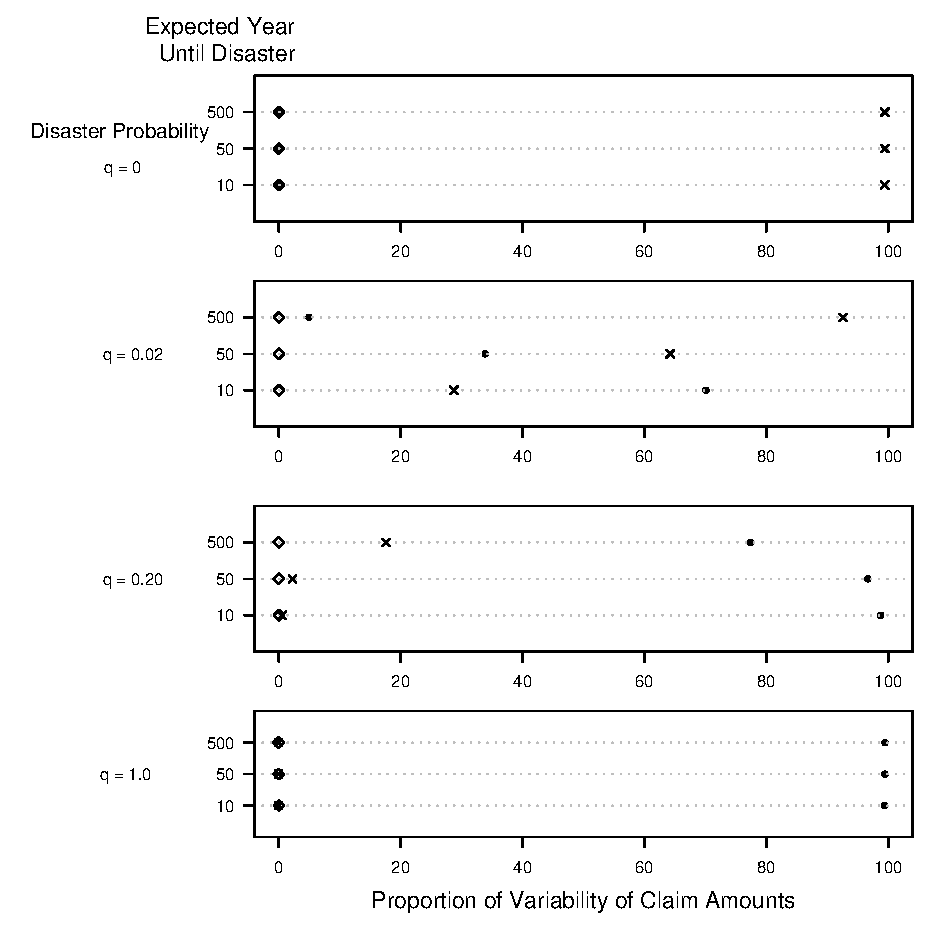
\includegraphics[width=0.8\textwidth]
        {Chapter21Graphs/Fig21_8MultipleDotPlots.eps}
  \includegraphics[width=0.1\textwidth]
        {Chapter21Graphs/Fig21_8Legend.eps}
    \caption{\label{F21:MultipleDotPlots} \small The Relative Importance of Risk Sources. This complex graph allows
us to visualize differences over sources of risk (interest, disaster
and mortality), expected year until disaster, and probability of
disaster. The multiway dot plot demonstrates how quickly the
importance of the disaster component increases as the probability of
disaster increases.}
  \end{center}
\end{figure}

Figure \ref{F21:MultipleDotPlots} shows that when no policyholders
succumb to disaster ($q = 0$), then the frequency component,
mortality, dominates the other risk sources. At the opposite
extreme, when all policyholders succumb to disaster ($q = 1$), then
the disaster component dominates the other risk factors. This is
true even when the expected time until disaster is 500 years! For
the intermediate cases, when either the expected proportion of
policyholders succumbing to disaster increases or the expected year
until disaster decreases, the importance of the disaster component
increases at the expense of the mortality component. Because of the
short-term nature of the contract considered, the interest component
does not play an important role in Figure
\ref{F21:MultipleDotPlots}.

This story of relative importance could not be told using analytic
expressions because of the complexity of the underlying models. The
story behind Figure \ref{F21:MultipleDotPlots} could be told,
however, using tabular displays. The advantage of Figure
\ref{F21:MultipleDotPlots} is that it allows the viewer to make
comparisons over three different risk sources when two parameters of
interest vary. Although such comparisons are possible with tabular
displays, graphical displays are more effective devices.

\linejed

\subsubsection*{Guideline Three: Use Complex Graphs to Portray Complex Patterns}

Many authors believe that a graph should be simple and immediately
understood by the viewer. Simple graphs are desirable because they
can deliver their message to a broad audience and can be shown
quickly and digested immediately. Although this notion may be
appropriate for popular writing, for professional writing the
concept of instant understanding is limiting in that it precludes
the notion that graphs demonstrate complex ideas. Complex patterns
should be portrayed as simply as possible, although the patterns
themselves should not be unnecessarily simplified.

One way for a graph to represent complex patterns is for some of its
basic elements to serve more than one purpose. Tufte (1983) called
such elements \emph{multifunctioning}. For example, we can use
plotting symbols to represent not only elements corresponding to the
horizontal and vertical scales but also a level of a categorical
variable.

\empexjed{WiscHospCosts} \index{datasets!Wisconsin hospital costs}

\linejed\index{actuarial \& financial terms and concepts!health
provider!fee for service, FFS} \index{actuarial \& financial terms
and concepts!health provider!health maintenance organization, HMO}

\textbf{Example \ref{S21:DesignGuide}.3: Frequency and Severity of
Hospital Costs}. Figure \ref{F21:PlotsLogCostDischarge} displays the
relationship between average hospital costs and frequency of
hospital usage. These data for the year 1989 were obtained from the
Office of Health Care Information, Wisconsin's Department of Health
and Human Services, and are further analyzed in Section 4.4. The
data represent averages over the state of Wisconsin, broken down by
nine health service areas, three types of providers (fee for
service, health maintenance organization, and other) and three types
of diagnosis-related groups (DRGs). The three DRGs, numbers 209, 391
and 430, represent major joint and limb reattachment, normal
newborns, and psychoses, respectively. Each plotting symbol in
Figure \ref{F21:PlotsLogCostDischarge} represents a combination of
health service area, type of payer, and type of DRG. The horizontal
axis provides the number of patients admitted in 1989 for each
combination, in natural logarithmic units. The vertical scale
provides the average hospital cost per discharge for each
combination, in natural logarithmic units.

The story in the left-hand panel, Figure
\ref{F21:PlotsLogCostDischarge}(a), is one of increased economies of
scale. That is, combinations of health service areas, type of payer,
and DRG that have a larger number of patients, measured by
discharges, have lower costs. A substantial negative relationship is
evident in Figure \ref{F21:PlotsLogCostDischarge}(a); the
correlation coefficient is -0.43. This is true despite the aberrant
point in the lower left-hand region of Figure
\ref{F21:PlotsLogCostDischarge}(a). The aberrant point is less
important economically than the others; it represents a combination
with only two discharges. When the point is removed, the correlation
becomes -0.50, thus representing an even stronger negative
relationship.

\begin{figure}[htp]
  \begin{center}\subfloat[\textbf{With the exception of one outlying
observation in the lower left-hand region, there appears to be a
significant negative relationship between cost and number of
hospital discharges.}]{
   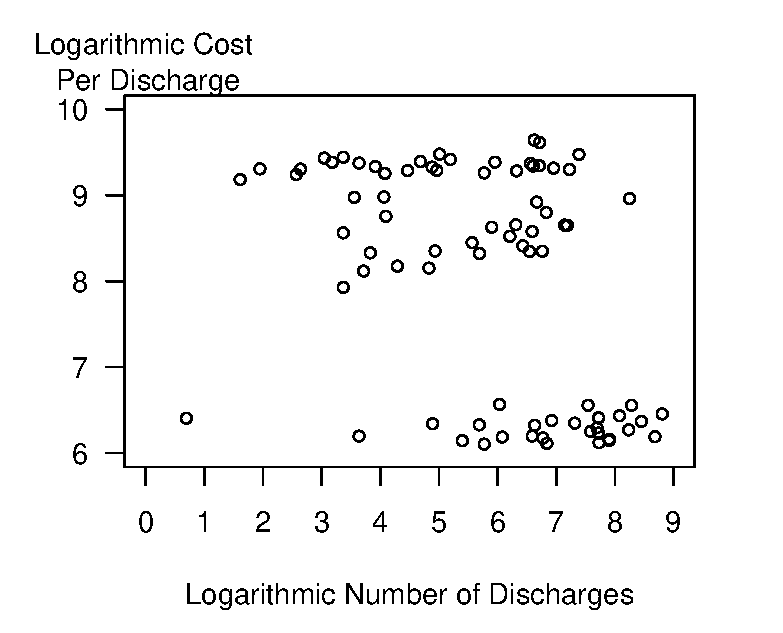
\includegraphics[width=0.45\textwidth]
   {Chapter21Graphs/Fig21_9PlotsLogCostDischargea.eps}}  \hfill
   \subfloat[\textbf{By introducing the DRG codes, we see a
small positive relationship between cost and number of hospital
discharges within each group.}]{
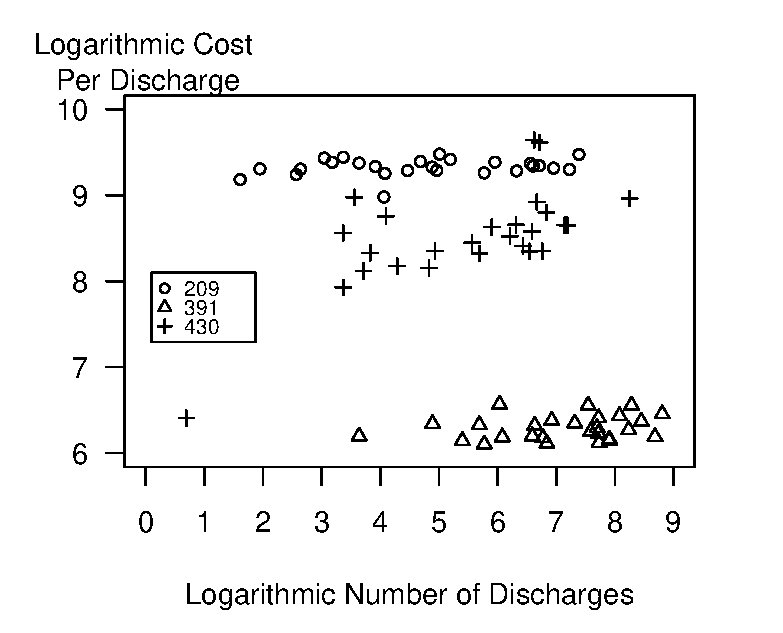
\includegraphics[width=0.45\textwidth]
        {Chapter21Graphs/Fig21_9PlotsLogCostDischargeb.eps}}
    \caption{\label{F21:PlotsLogCostDischarge} \small Logarithmic Cost per Discharge Versus the Logarithmic Number of
Discharges. By adding a plotting symbol code for the level of DRG,
the three distinct groups are evident. The three DRGs, 209, 391, and
430, represent major joint and limb reattachment, normal newborns
and psychoses, respectively.}
  \end{center}
\end{figure}


Despite its simplicity, Figure \ref{F21:PlotsLogCostDischarge}(a)
hides an important relationship. The right-hand panel, Figure
\ref{F21:PlotsLogCostDischarge}(b), is a redrawing of Figure
\ref{F21:PlotsLogCostDischarge}(a) that includes different plotting
symbols for different DRGs. Here, the story is the opposite to the
one of increased economies of scale. For combinations representing
major joint and limb reattachments and normal newborns, the
relationship between frequency and cost is fairly flat. For these
DRGs there are few economies of scale. For the psychoses DRG, number
430, Figure \ref{F21:PlotsLogCostDischarge}(b) shows a small
positive relationship between frequency and cost, even discounting
for the combination with only two patients discharged.

The two panels illustrate a phenomenon in statistics referred to as
\emph{Simpson's paradox}, or a problem of \emph{aggregation of
data}. See Section 4.4 for further discussion. The important point
for this chapter is that sometimes simple graphs are misleading.
Complex graphs may take more time for viewers to interpret, but they
more effectively summarize complex relationships.

\linejed

\subsubsection*{Guideline Four: Relate Graph Size to Information Content}

``How large should the graph be?'' is an important question. The
bounds on size are clear. Graphs should not be so small that they
are not clearly legible, particularly upon reproduction that
degrades an image, nor should they be so large that they exceed a
page. With large graphs, it is difficult to compare elements within
the graph, thus defeating a primary purpose of graphs.

\marginparjed{The data density of a graph is the number of data
entries per unit area of the graph.}\index{plots!data density}

Within these bounds, a graph should be proportional to the amount of
information that it contains. To discuss the proportion of
information content, Tufte (1983) introduced the \emph{data density
of a graph}. This is defined to be the number of data entries per
unit area of the graph. For comparing graph size and information,
the data density is a quantity to be maximized, either by increasing
the number of data entries or reducing the size of the graph. By
examining this density over a number of popular publications, Tufte
concluded that most graphs could be effectively shrunk.

For example, Figure \ref{F21:DotPlotPremiumReceipts}(a) is a chart
with a low data density. This chart represents only 15 numbers. With
an area of approximately 9 square inches, this graph's data density
is roughly 15/9. For comparison, Figure
\ref{F21:InflationWithProjections} shows approximately 600 numbers.
Although Figure \ref{F21:InflationWithProjections}'s area is about
twice as large as that of Figure
\ref{F21:DotPlotPremiumReceipts}(a), the data density is much larger
in Figure \ref{F21:InflationWithProjections} than in Figure
\ref{F21:DotPlotPremiumReceipts}(a).


\begin{figure}[htp]
  \begin{center}
    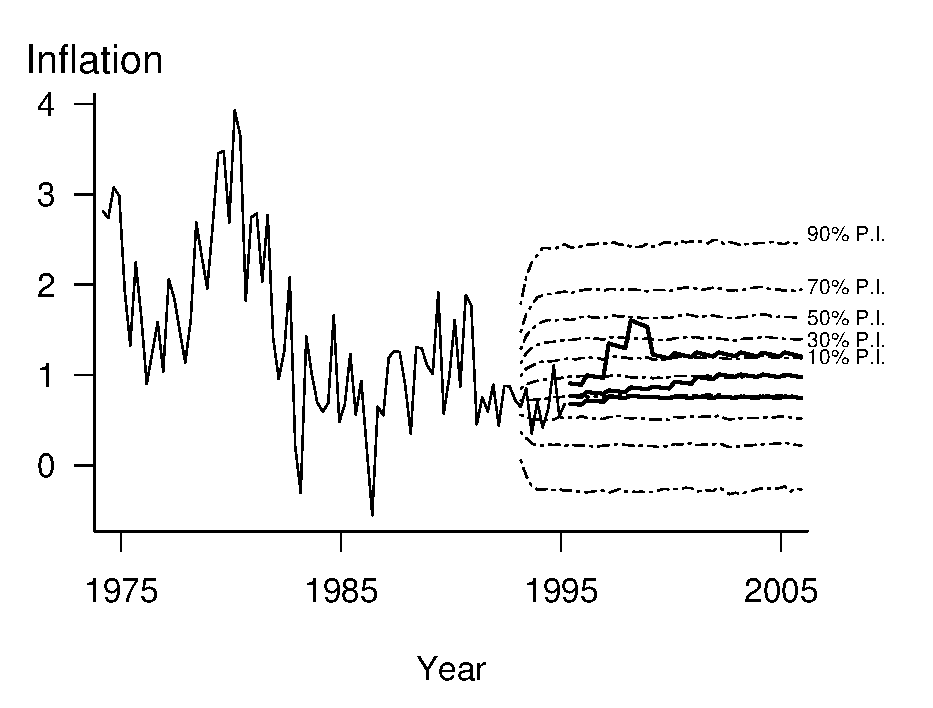
\includegraphics[width=0.9\textwidth]
        {Chapter21Graphs/Fig21_10InflationWithProjections.eps}
    \caption{\label{F21:InflationWithProjections} \small Comparison of Stochastic Prediction Intervals to Held-out Actual
Experience and to Social Security's Assumptions. The thin solid
lines represent actual inflation rates, and the thick solid lines
represent projections by Social Security experts. The dotted lines
represent prediction intervals generated by a stochastic time series
model. This complex graph allows viewers to make comparisons based
on approximately 600 points.}
  \end{center}
\end{figure}

\linejed

\textbf{Example \ref{S21:DesignGuide}.4: Inflation Rate Forecasts}.
Figure \ref{F21:InflationWithProjections} is a complex graph that
contains much information about a complex subject, forecasting the
inflation rate (CPI) for projections of Social Security funds (Frees
et al. 1997). The graph shows actual experience of quarterly
inflation rates up through the first quarter of 1995. Experience up
through 1992 was used to fit a time series model described in Frees
et al. (1997), and this model was used to generate prediction
intervals (PIs) of the inflation rate. These prediction intervals
can be compared to held-out experience that was not used to fit the
model (1993-1995) as well as projections of inflation by Social
Security experts. The thick lines represent high-, intermediate-,
and low-cost inflation projections determined by Social Security
experts.

Figure \ref{F21:InflationWithProjections} is complex and may not be
immediately understood by the viewer. However, almost every stroke
within the data region represents numerical information. Although
complex, Figure \ref{F21:InflationWithProjections} allows the viewer
to compare (1) 20 years of experience to a 10-year forecast, (2)
recent held-out experience to forecasts, and (3) expert projections
to forecasts generated by a time series model. The graph's
complexity reflects the complexity of forecasting inflation rates;
this complexity is not due to unnecessary elements that distract
viewers and make them more ``interested'' in the graph.

\linejed

\subsubsection*{Guideline Five: Use Graphical Forms That Promote Comparisons}

Creators of graphs are often faced with the choice of several
graphical forms that could be used to represent a feature of the
data. As we describe in Guideline Eight, the receiver's knowledge of
graphical forms can influence the choice. Graphical perception is
also an important determinant. In Section
\ref{S21:EmpiricalFoundations}, we discuss this issue in detail. We
include it here as part of the Guidelines Section for completeness.

\subsubsection*{Guideline Six: Integrate Graphs and Text}


Data graphics should be carefully integrated with text, tables, and
other graphs. A legend summarizes the graph and its main message,
but the surrounding text develops the theme leading up to the
message and discusses its impact. Although ``a picture is worth ten
thousand words,'' a graph needs supporting text. Tufte (1983)
encourages readers and writers to think of data graphics as
paragraphs and to treat them as such.

Data graphics can be complemented by a tabular presentation of data:
graphics can highlight relationships among the data, and tables can
present precise numerical descriptions of the data. The two modes
are complementary. A good writing device is to place a graphical
display in the main body of the report and to reinforce the graph
with a tabular display in an appendix.

The American Statistical Association, in its \emph{Style Guide} for
journal publications, reminds us that a detailed legend is helpful
when interpreting graphs. The \emph{Style Guide} recommends that a
legend describe a graph, draw attention to the graph's important
features, and explain this importance.

\subsubsection*{Guideline Seven: Demonstrate an Important Message}

Detailed legends and graphs should reinforce messages that are
developed in the main body of the text. To illustrate, when
considering ways of portraying a complex dataset, choose a graphical
form that highlights an important message. All too often, creators
of graphs display data features that are not part of the theme that
is being developed.

Cleveland (1994) recommends that we ``put major conclusions in a
graphical form.'' In regression data analysis, major conclusions are
about patterns in the data that are summarized using models. Usually
major conclusions are best presented graphically. Graphs display a
large amount of information that is retained by the viewer because
it is visualized. Graphs communicate patterns directly to a viewer,
without using an equation to represent the patterns. In this way, a
wider audience can be reached than if the presentation relies solely
on a model-based interpretation of the data. Further, patterns
suggested by a graph reinforce those represented by a model, and
vice versa. Thus the two tools, graphs and models, reinforce and
strengthen one another.

\marginparjed{``The greatest value of a picture is when it forces us
to notice what we never expected to see.'' Tukey (1977)}

Tukey (1977) states that ``The greatest value of a picture is when
it forces us to notice what we never expected to see.'' Unexpected
phenomena are usually memorable events; viewers of graphs remember
these results, which makes them powerful. In writing this chapter,
we did not expect the results of Figure \ref{F21:tsUnemploy}. This
figure demonstrates that unemployment rises much more quickly than
it declines; it is a powerful example of the use of aspect ratios.

\subsubsection*{Guideline Eight: Know Your Audience}

A basic precept of effective writing, familiarity with one's
audience, is also valid for designing effective graphs. As stated in
the Introduction, our primary motivation in developing guidelines is
to encourage the precise and concise communication of quantitative
ideas to a scientific audience using a written medium. As discussed
in Section \ref{S21:EmpiricalFoundations}, the graphical form is
subservient to the real role of the graphical display,
\emph{communicating} quantitative ideas of the creator to the viewer
of a graph. If the audience does not have an understanding of the
graphical form, then the form will hinder the communication flow
rather than aid it. Thus, each of the seven guidelines already
discussed can be modified or even ignored upon occasion, depending
on the audience for the graph. To illustrate, in Example
\ref{S21:DesignGuide}.1 we argued that the dot plot was superior to
the three-dimensional stacked bar chart. As another example, in
Section \ref{S21:EmpiricalFoundations} we argue that pie charts are
ineffective communicators of information based on the science of
cognitive perception. However, for some audiences, creators of
graphs will prefer the less effective forms based on the level of
audience familiarity. We hope that practice will eventually shift
from these ineffective modes of communication. Still, it is
important to recognize the background of the audience of the graph.
We recommend that creators of graphs not so much swim against the
tide of poor graphic design as bend their course towards more
effective modes of communication.


\section{Empirical Foundations For
Guidelines}\label{S21:EmpiricalFoundations}

This section consists of two different scientific aspects of
graphical studies: science of perception and surveys of graphical
practice.

This chapter does not include a number of graphical forms that are
mainstays in business publications and the popular press, such as
pie charts, pictographs, and stacked bar charts. In fact, we have
shown stacked bar charts in Section \ref{S21:DesignGuide} only as an
example of how \emph{not} to draw figures. Why are these widely used
graphical forms not adopted in an chapter emphasizing data graphics?
The reasons lie in how graphical forms communicate information and
how we perceive graphical information. We demonstrate that, given
how we perceive information, pie and stacked bar charts are poor
communicators of numerical information.

As described in Section \ref{S21:Intro}, data graphics encode
information, and we, as viewers, decode this information when
viewing a graph. The efficiency of this transmission can be
considered in the context of cognitive psychology, the science of
perception. This discipline provides a framework for distinguishing
among different types of information processing that we do when
decoding graphs. Identifying different types of information
processing will help us decide what are effective, and ineffective,
graphical forms.


\subsection{Viewers as Units of Study}

Table \ref{T21:GraphPerception} is an ordered list of basic
graphical perception tasks, according to Cleveland (1994). Here, the
ordering begins with a set of tasks that is least difficult for a
viewer to perform and ends with a set that is most difficult. Thus,
for example, judging position along a common scale is the least
difficult for viewers and judging relative shadings of colors and
density (the amount of ink) is the most difficult.


%\boxedjed

\begin{table}[h]
\caption{\label{T21:GraphPerception} Basic Graphical Perception
Tasks}
\begin{tabular}{l}\hline
1. Position along a common scale \\
2. Position along identical, nonaligned scales \\
3. Length \\
4. Angles and slopes \\
5. Area \\
6. Volume \\
7. Color and density \\\hline
\end{tabular}
\end{table}

%\end{boxedminipage}


To understand the relative difficulty of the tasks, Cleveland and
McGill (1984) performed a series of tests on many experimental
subjects. To illustrate, Figures
\ref{F21:11aExperiments}-\ref{F21:11cExperiments} presents a series
of tests that are analogous to the first five tasks. Cleveland and
McGill summarized the performance of the experimental subjects by
calculating the accuracy with which the subjects performed each set
of tasks. Through these measures of relative accuracy, and arguments
from cognitive psychology, Cleveland and McGill developed the
ordering presented in Table \ref{T21:GraphPerception}.


\begin{figure}[htp]
  \begin{center}
  \subfloat[\textbf{Experiment
to Judge Position along a Common Scale. Assess the relative values
of A, B, C and D along this 100-point scale.}]{
   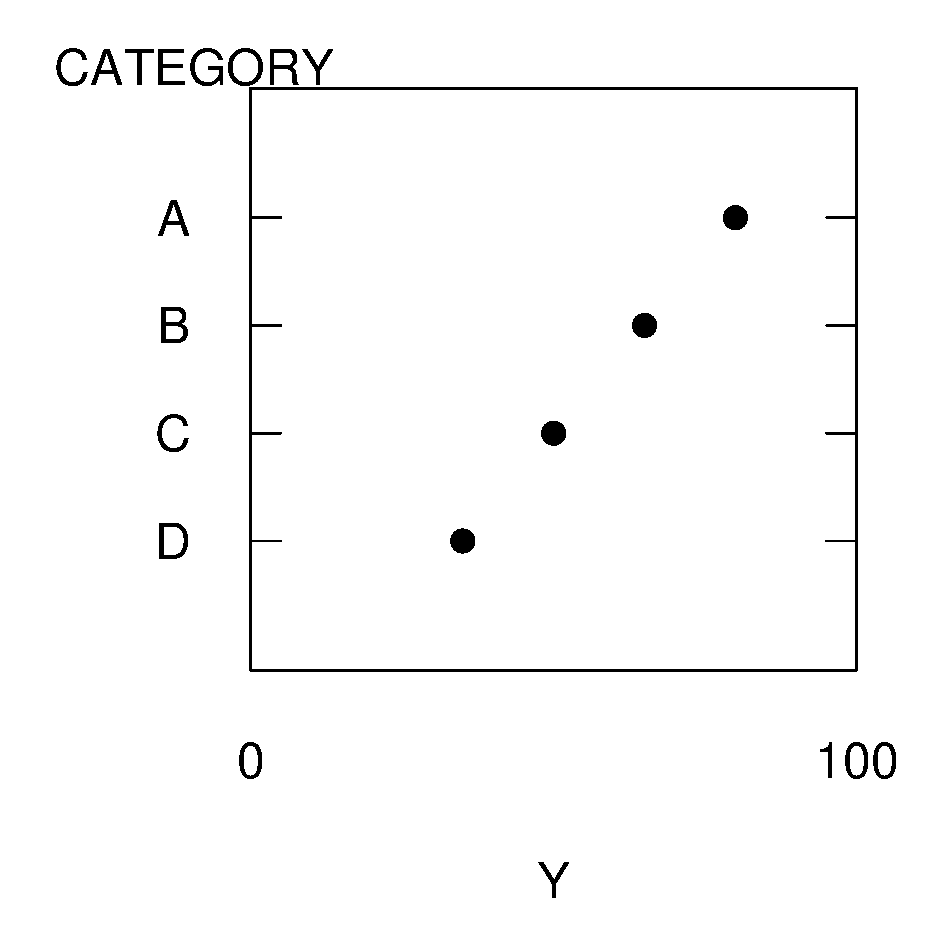
\includegraphics[width=0.35\textwidth]
   {Chapter21Graphs/Fig21_11aExperiments.eps}} \newline
  \subfloat[\textbf{Experiment to Judge Position along Identical, Nonaligned Scales.
Assess the relative values of A, B, C and D on a common 100-point
scale.}]{
   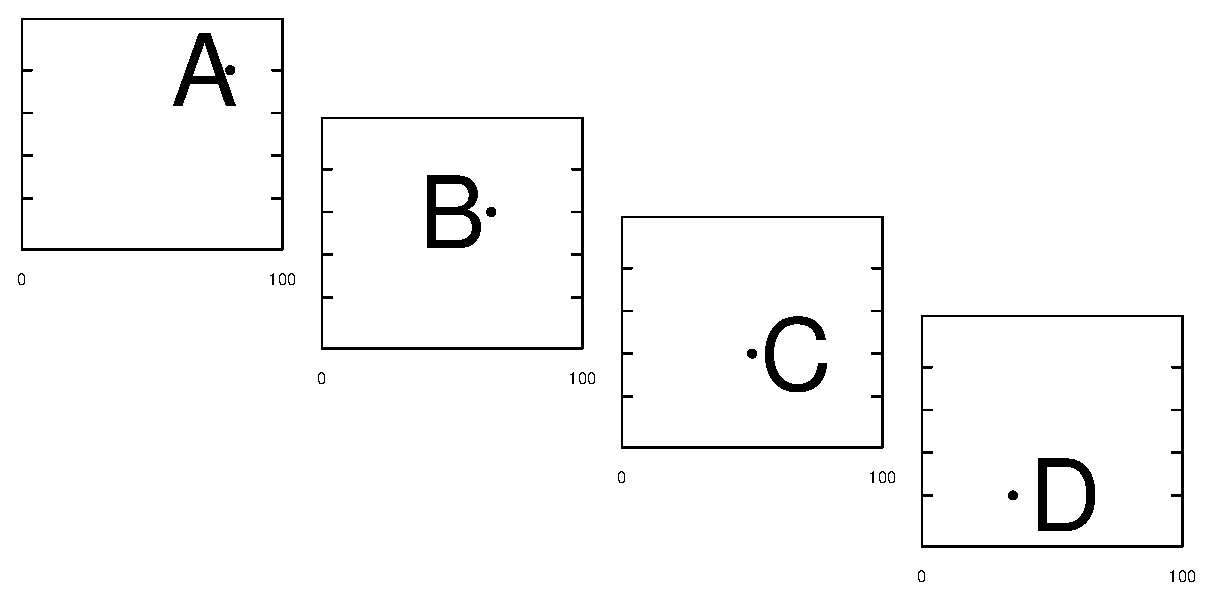
\includegraphics[width=0.53\textwidth]
   {Chapter21Graphs/Fig21_11bExperiments.eps}}  \hfill
   \subfloat[\textbf{Experiment to Understand Length Judgments. Suppose line A
is 100 units long. Assess the relative lengths of lines B, C and
D.}]{
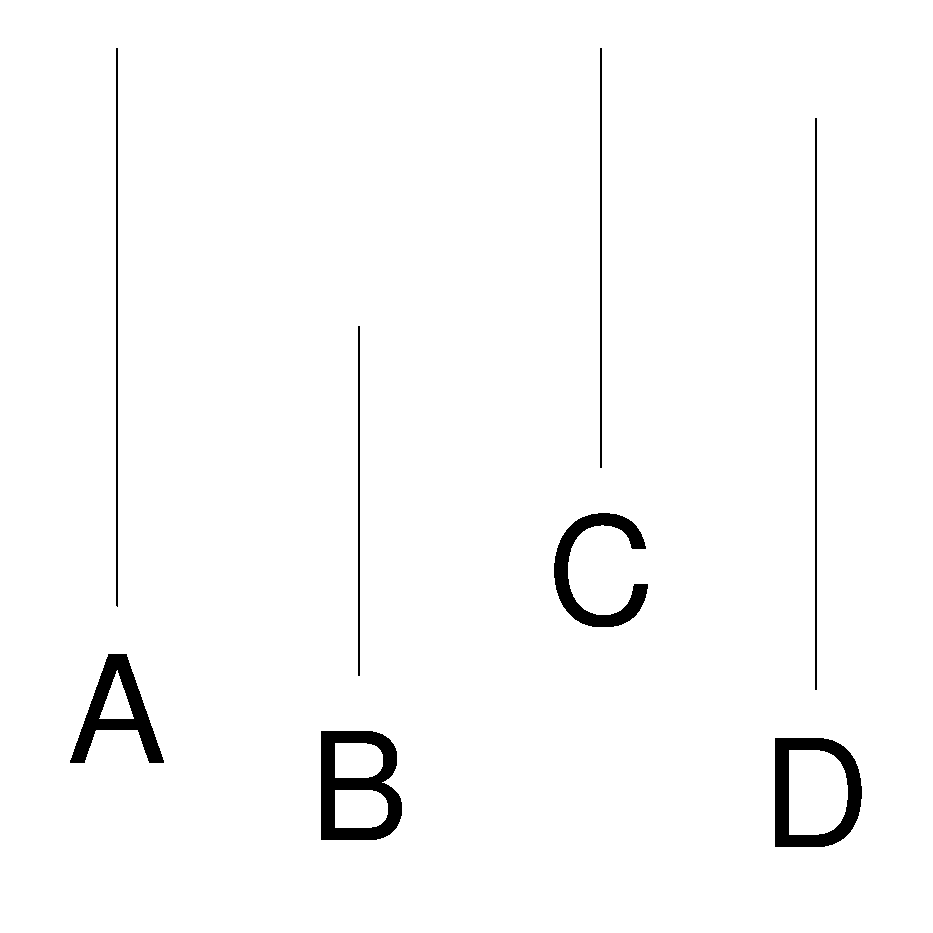
\includegraphics[width=0.3\textwidth]
        {Chapter21Graphs/Fig21_11cExperiments.eps}}
 \subfloat[\textbf{Experiment to
Understand Angle Judgments. Suppose angle A is 100 units. Assess the
relative  values of angles B, C and D.}]{
   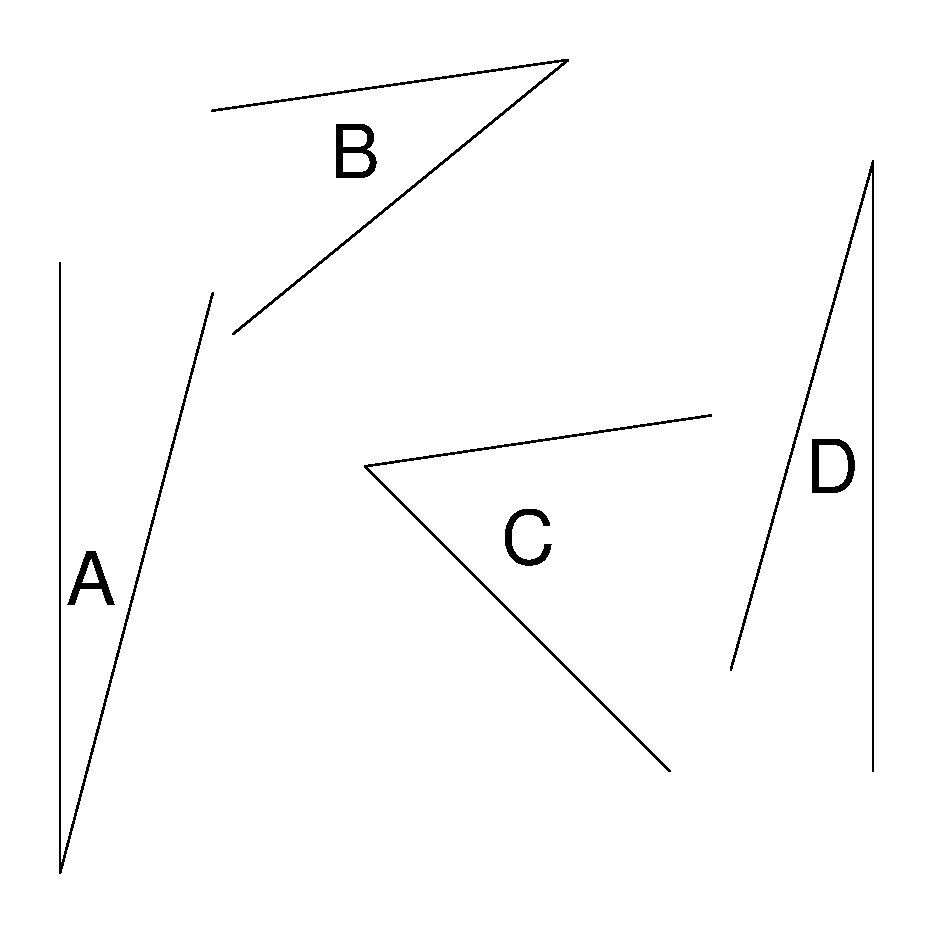
\includegraphics[width=0.45\textwidth]
   {Chapter21Graphs/Fig21_11dExperiments.eps}}  \hfill
   \subfloat[\textbf{Experiment to Understand
Area Judgments. Suppose circle A has area 100 units. Assess the
relative areas of circles B, C and D.}]{
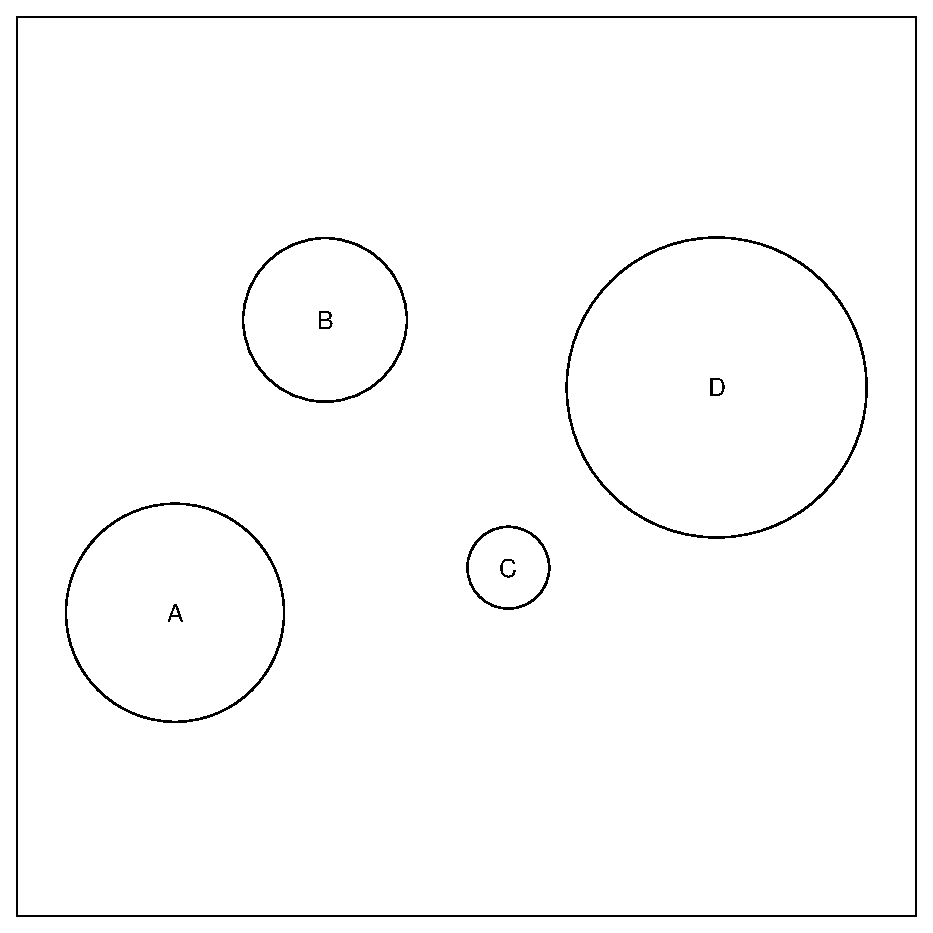
\includegraphics[width=0.45\textwidth]
        {Chapter21Graphs/Fig21_11eExperiments.eps}}
    \caption{\label{F21:11aExperiments} \small Experiments in Judgments about Graphical Perception}
  \end{center}
\end{figure}



This chapter does not discuss the use of color because of the
complexities of coding and decoding it effectively. We refer
interested readers to Cleveland (1994, Section 3.13) and Tufte
(1990, Chapter 5) for further information.

The ordered list of graphical perception tasks can help the creator
choose the appropriate graphical form to portray a dataset. When
confronted with a choice of two graphical forms, a creator should
select the form that is least difficult for the viewer. Other things
being equal, a task that can be performed with little difficulty by
the viewer means that information can be transmitted more reliably.
To illustrate, we discuss two examples in which Table
\ref{T21:GraphPerception} can help you decide on the appropriate
graphical form for portraying a dataset.

\linejed

\textbf{Example \ref{S21:EmpiricalFoundations}.1: Distribution of
Premium Income}. The first example demonstrates some shortcomings of
the stacked bar chart. For this discussion, we return to Example
\ref{S21:DesignGuide}.1. Figure \ref{F21:DotPlotPremiumReceipts}(a)
is a three-dimensional stacked bar chart. We have already discussed
the substantial amount of chartjunk in this figure. Even without the
useless pseudo third dimension, the stacked bar chart requires the
viewer to make length judgments to understand, for example, the
distribution of annuity receipts over time. In contrast, the dot
plot in Figure \ref{F21:DotPlotPremiumReceipts}(b) requires the
viewer to make comparisons only according to positions along a
common scale. As described in Table \ref{T21:GraphPerception}, the
latter is an easier task, resulting in more reliable information for
the viewer. Thus, we conclude that the dot plot is preferred to the
stacked bar chart.

\linejed

\textbf{Example \ref{S21:EmpiricalFoundations}.2: Distribution of
Mortgages}. Our second example demonstrates the inadequacy of pie
charts. Figure \ref{F21:PieChartsMortgages} is an adaptation of the
figure on page 100 of the \emph{Life Insurance Fact Book} (1994). It
reports, for the years 1973, 1983 and 1993, commercial, 1- to
4-family, and farm mortgages as percentages of total mortgages. Pie
charts make comparisons difficult. For example, the graph makes it
difficult to detect whether farm mortgages are more prevalent than
1- to 4-family mortgages in 1983, or whether farm mortgage
percentages increased or decreased from 1973 to 1983. The comparison
of percentages across years is a linear operation, yet the pie
charts require us to decode angles, a difficult task according to
the ordering in Table \ref{T21:GraphPerception}. As with Example
\ref{S21:DesignGuide}.1, the charts in Figure
\ref{F21:PieChartsMortgages} make things worse by reporting in three
dimensions; these figures not only require us to decode volumes but
also add substantially to the chartjunk in the graphic. \emph{Only
nine numbers are reported in this graphic}, three years and two
percentages in each year. (The third percentage can be computed by
subtraction.)


\begin{figure}[htp]
  \begin{center}
    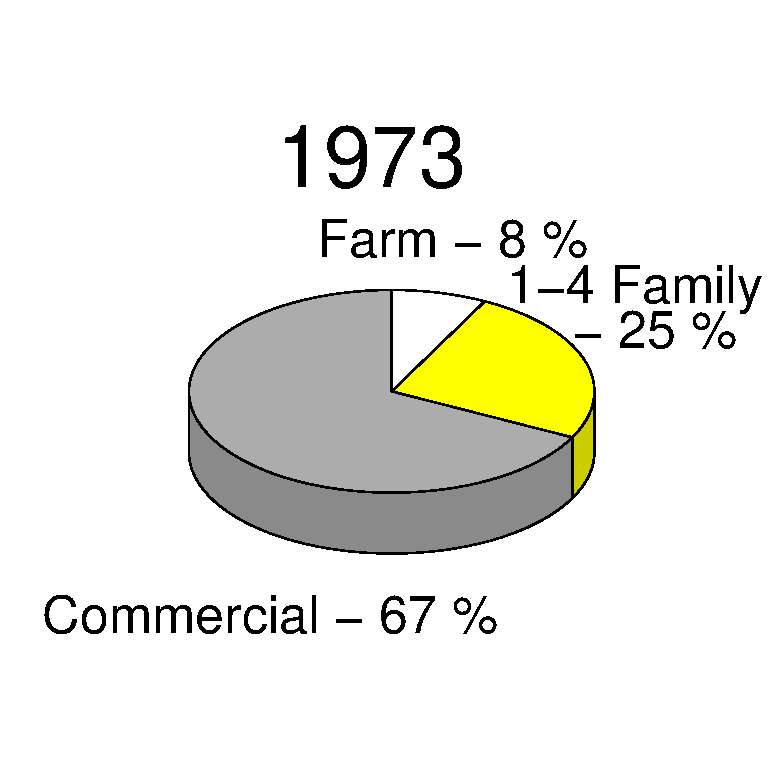
\includegraphics[width=0.31\textwidth]{Chapter21Graphs/F21Mortgage73.eps}
    \hfill
        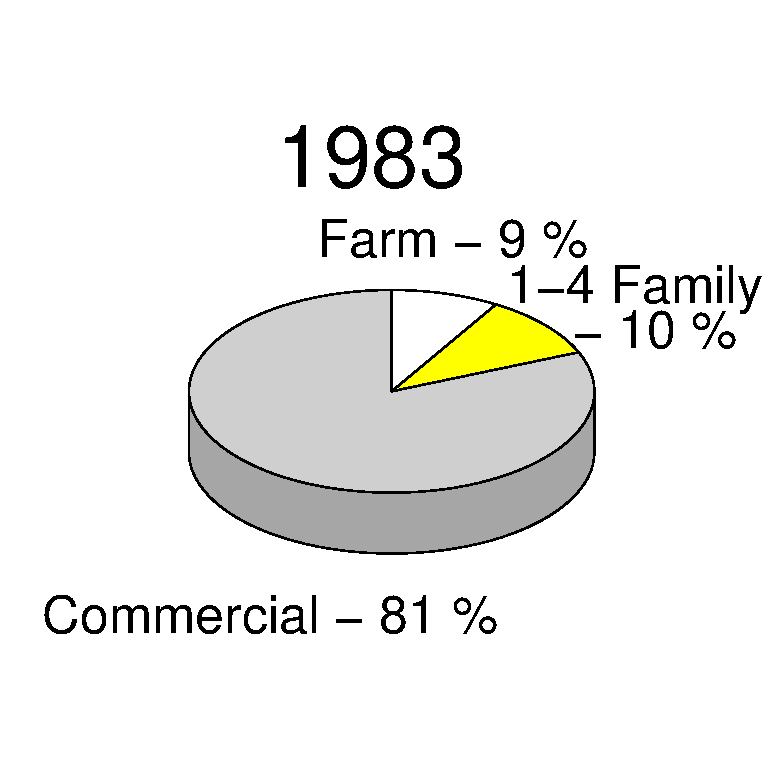
\includegraphics[width=0.31\textwidth]{Chapter21Graphs/F21Mortgage83.eps} \hfill
            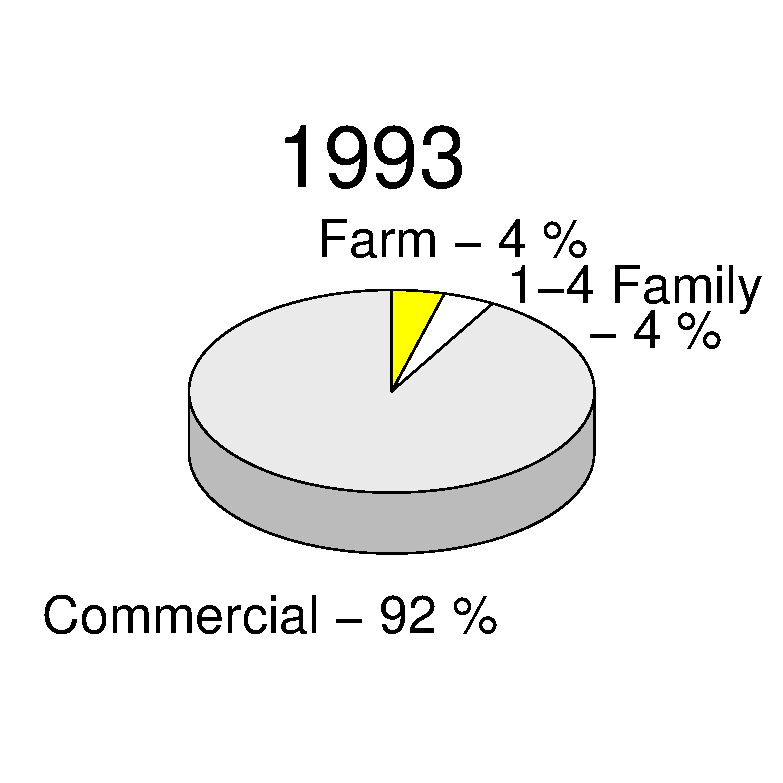
\includegraphics[width=0.31\textwidth]{Chapter21Graphs/F21Mortgage93.eps}
    \caption{\label{F21:PieChartsMortgages} \small Distribution of Mortgages for the Years 1973, 1983 and
1993. The three-dimensional pie chart is a poor graphical form for
making comparisons over time and across types of mortgages.}

  \end{center}
\end{figure}

If a graphic is needed, then the dot plot in Figure
\ref{F21:DotPlotPerCentMortgages} is more than sufficient. Here,
comparisons are made according to positions along a common scale, a
task easier than comparing angles. Pie charts require us to make
comparisons using angles, which are more difficult and less reliable
than comparisons using other graphical forms.

\begin{figure}[htp]
  \begin{center}
    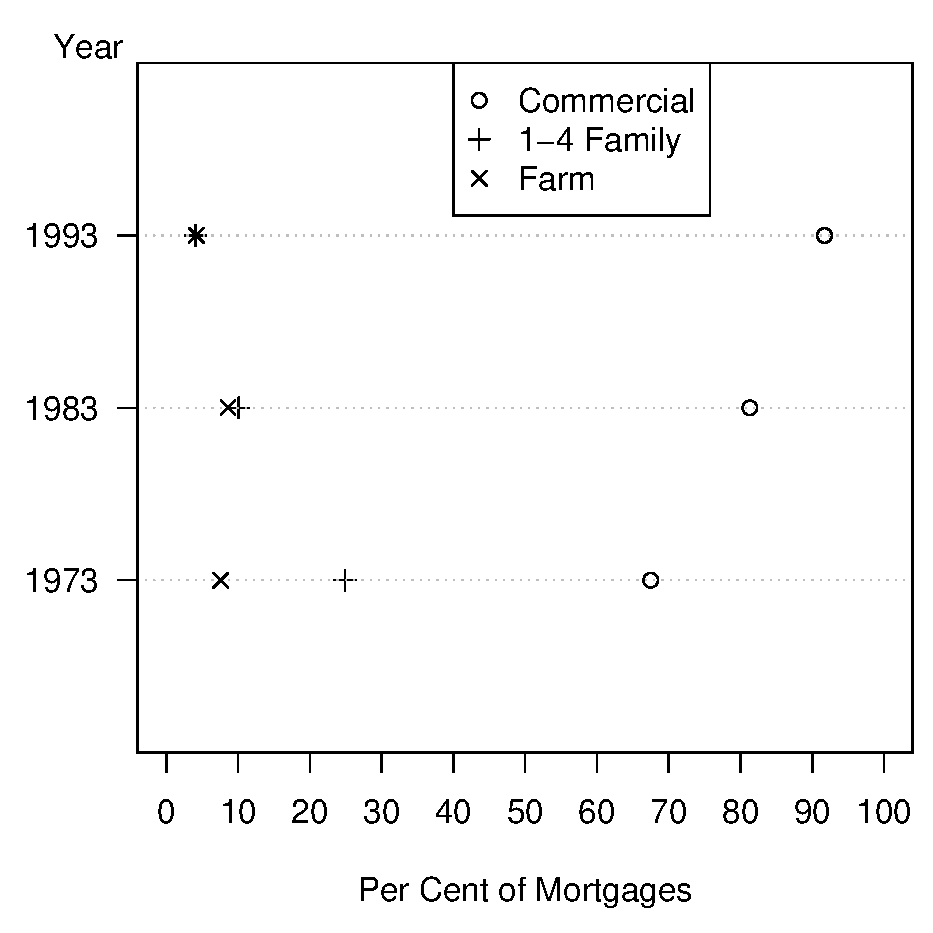
\includegraphics[width=0.5\textwidth]
        {Chapter21Graphs/Fig21_13DotPlotPerCentMortgages.eps}
    \caption{\label{F21:DotPlotPerCentMortgages} \small Commercial, 1- to 4-Family, and Farm Mortgages as
Percentages of Total Mortgages for 1973, 1983 and 1993. A negative
aspect of this graph is the overlap of the 1- to 4-family and farm
plotting symbols in 1983 and 1993.}
  \end{center}
\end{figure}

Although Figure \ref{F21:DotPlotPerCentMortgages} is a more
effective graph than Figure \ref{F21:PieChartsMortgages}, for these
data we recommend a tabular display (Table \ref{T21:Mortgages}),
which allows for clear comparisons across mortgage types and across
years. Further, more detailed information about mortgage percentages
is available in Table \ref{T21:Mortgages} than in Figure
\ref{F21:PieChartsMortgages} or \ref{F21:DotPlotPerCentMortgages}.
Of course, we can always superimpose the actual percentages, as is
often done with pie charts and as illustrated in Figure
\ref{F21:PieChartsMortgages}. Our response to this approach is to
question the worth of the entire graph. As with writing, each stroke
should offer new information; let creators of graphs make each
stroke tell!

\linejed

\subsection{Graphs as Units of Study}

Surveys of graphical practice in professional publications provide
an important database with which to assess prevalence of good and
bad practice and changes in practice over time. Tufte (1983, pp. 82-
86) discusses a survey of approximately 4,000 graphs randomly
selected from 15 news publications for the years 1974 to 1980. The
graphs were assessed for ``sophistication,'' defined as presentation
of relationship between variables, excluding time series or maps.
Cleveland and McGill (1985) report a similar survey of scientific
publications, assessing the prevalence of graphical errors.

\begin{table}[h] \scalefont{0.9}
\caption{\label{T21:Mortgages} Commercial, 1- to 4-Family, and Farm
Mortgages \newline as Percentages of Total Mortgages for 1973, 1983,
1993}
\begin{tabular}{lrrr}
\hline
 & \multicolumn{3}{c}{Year}\\
\hline Mortgage Type
 & 1973 & 1983 & 1993 \\ \hline
Commercial & 67.5 & 81.3 & 91.7 \\
1-4 Family & 24.9 & 10.1 & 4.1 \\
Farm & 7.6 & 8.6 & 4.2 \\ \hline
\end{tabular}
\scalefont{1.1111}
\end{table}

Harbert (1995) assessed every graph and table in the 1993 issues of
four psychology journals on 34 measures of quality. The measures of
quality were gleaned from the current research literature on graphic
quality. They were converted into a check sheet, and a check sheet
was filled out for each graph and table in the selected psychology
journals. Harbert's study yielded data on 439 graphs and tables. We
summarize the analysis of the 212 graphs.

Harbert assigned letter grades to the graphics: A, AB, B, BC, C, CD,
D, DF and F. These grades reflected her overall evaluation of the
graphs as communicators of statistical information. The grades were
converted to numerical values: 4.0, 3.5, 3.0, 2.5, 2.0, 1.5, 1.0,
0.5 and 0.0. The numerical values were the dependent variable in a
regression. The independent variables were the 34 measures of
quality, suitably coded. The purpose of the study was to determine
which factors were statistically significant predictors of the
grades assigned by an ``expert'' evaluator of graphics. By trial and
error, Harbert selected a multiple linear regression equation in
which all the predictors were statistically significant (5\% level)
and no other predictors achieved this level of significance when
added to the equation. Table \ref{T21:Factors} shows the variables
included in the regression equation ($R^2 = 0.612$).



\begin{table}[h] \scalefont{0.9}
\caption{\label{T21:Factors} Factors Affecting Assessment of Graphic
Quality, \newline ~Harbert Study}
\begin{tabular}{ll}
\hline
Variables with & Variables with\\
Positive Coefficients & Negative Coefficients \\ \hline Data-ink
ratio
& Proportion of page used by graphic\\
Comparisons made easy &Vertical labels on Y-axis \\
Sufficient data to make  &Abbreviations used \\
~~~a rich graphic&Optical art used \\
&Comparisons using areas or volumes \\
\hline
\end{tabular}
\scalefont{1.1111}
\end{table}



Data-ink ratio was defined by Tufte (1983, p. 93) as the
``proportion of the graphics ink devoted to the nonredundant display
of data-information'' or equivalently as ``1.0 minus the proportion
of a graphic that can be erased without loss of data-information.''
The data-ink ratio is more readily calculated than the data density
measure defined in Section \ref{S21:DesignGuide} of this paper.
Optical art is decoration that does not tell the viewer anything
new.

One variable that had been anticipated as very significant was data
density, which is difficult and time-consuming to measure. An
important finding of the study was that the easier-to-measure
data-ink ratio and proportion of page variables were sufficient to
predict the grades. A quotation from Harbert's thesis sums up the
finding: ``The highest grades were given to those graphics that take
up small proportions of the page, have a large data-ink ratio, make
comparisons easy, have enough data points, have horizontally printed
labels, do not have abbreviations, do not have optical art, and do
not use volume or 3-D comparisons'' (Harbert 1995, p. 56).

As a small follow-up study to Harbert's work, we examined each of
the 19 non-table graphics in the \emph{Life Insurance Fact Book}
(1994), assessing them on seven negative factors. Table
\ref{T21:GraphsFactors} shows the percentage of graphs that
displayed each of the negative factors.


\begin{table}[h] \scalefont{0.9}
\caption{\label{T21:GraphsFactors} Percentage of Graphs Displaying
Negative Factors \newline in Life Insurance Fact Book 1994}
\begin{tabular}{lc}
\hline
 Negative Factor &Percentage \\ &of Graphics \\ \hline Use of 3-D bars & ~~~79 \%
 \\
Grid lines too dense &79 \\
 Making comparison of time series values
hard &37\\
 Use of stacked bars & 37 \\
 Growth displayed poorly &32\\
 Use of
lines that are wider than need be& 16\\ Use of pies &5\\ \hline
\end{tabular}
\scalefont{1.1111}
\end{table}




Our review suggests that every graphic could have been reduced by
50\% to 75\% without loss of clarity. This observation is in keeping
with Harbert's finding about the proportion-of-page variable. In a
word, the graphs in the \emph{Life Insurance Fact Book} could be
produced much more ably. Doing so would improve the quality of
communication and would potentially increase the respect with which
knowledgeable professionals in other fields view the insurance
industry.

We hope that other investigators will engage in further study of
graphic practice in actuarial publications. By using data from such
studies, the profession can improve its practice, making
communications efficient and precise.

\section{Concluding Remarks}\label{S21:Conclude}

The Society of Actuaries' motto is a quotation of Ruskin: ``The work
of science is to substitute facts for appearances and demonstrations
for impressions.'' Armed with the guidelines outlined in this paper
and discussed further in the references, actuaries can be leaders in
presenting data graphically, thus substituting demonstrations for
impressions. Surveys of recent actuarial literature should be the
basis for assessing current practice. Editors and referees of
professional publications can be especially influential in bringing
about a rapid improvement in standards of practice. Moreover,
actuaries can recommend and use statistics textbooks that pay
attention to graphic quality.

Because actuaries read material that contains graphs, they are
consumers. They should become tough customers! All too often the
defaults in spreadsheet and statistical graphics software become the
norm. Actuaries should not allow the choices made by software
programmers to drive graphic quality or standards. Although it is
easy to create graphs using defaults in the graphics software, the
resulting graphs are seldom fully satisfactory. If a graph is not
worth doing well, let's leave it out of our publications.


\section{Further Reading and References}\label{S21:References}

In addition to the references listed, other resources are available
to actuaries interested in improving their graphic design skills.
Like the Society of Actuaries, another professional organization,
the American Statistical Association (ASA), has special interest
sections. In particular, the ASA now has a section on statistical
graphics. Interested actuaries can join ASA and that section to get
the newsletter \emph{Statistical Computing \& Graphics}. This
publication has examples of excellent graphical practice in the
context of scientific discovery and application.

The technical \emph{Journal of Computational and Graphical
Statistics} contains more in-depth information on effective graphs.
We also recommend accessing and using the \emph{ASA Style Guide }at
http:
//www.amstat.org/publications/style-guide.html as an aid to
effective communication of quantitative ideas.

\bigskip

\textbf{Chapter References}

\begin{multicols}{2}

\scalefont{0.9}

American Council of Life Insurance. Various years. \emph{Life
Insurance Fact Book}. Washington, D.C.: ACLI.

Cleveland, William S. (1994). \emph{The Elements of Graphing Data}.
Monterey, Calif.: Wadsworth.

Cleveland, William S. (1993).  \emph{Visualizing Data}. Summit,
N.J.: Hobart Press.

Cleveland, William S., Diaconis, P., and McGill. R. (1982).
Variables on scatterplots look more highly correlated when the
scales are increased. \emph{Science} 216, 1138-1141.

Cleveland, William S., and McGill, R. (1984). Graphical perception:
Theory, experimentation, and application to the development of
graphical methods. \emph{Journal of the American Statistical
Association} 79, 531-454.

Cleveland, William S., and McGill, R. (1985). Graphical perception
and graphical methods for analyzing and presenting scientific data.
\emph{Science} 229, 828-833.

Ehrenberg, A.S.C. (1977). Rudiments of Numeracy. \emph{Journal of
the Royal Statistical Society A} 140:277-97.

Frees, Edward W. (1996). \emph{Data Analysis Using Regression
Models.} Englewood Cliffs, N.J.: Prentice Hall.

Frees, Edward W. (1998). Relative Importance of Risk Sources in
Insurance Systems, \emph{North American Actuarial Journal} 2(2),
34-51.

Frees, Edward W., Kung, Yueh C., Rosenberg, Marjorie A., Young,
Virginia R., and Lai, Siu-Wai (1997). Forecasting Social Security
Assumptions, \emph{North American Actuarial Journal} 1(3), 49-82.

Harbert, D. (1995). The Quality of Graphics in 1993 Psychology
Journals, Senior honors thesis, University of Wisconsin-Madison.

Huff, D. (1954). \emph{How To Lie with Statistics}. New York:
Norton.

Schmid, C.F. (1992). \emph{Statistical Graphics: Design Principles
and Practices} Malabar, Fla.: Krieger Publishing Co.

Schmit, Joan T., and Roth, K. (1990). Cost Effectiveness of Risk
Management Practices, \emph{Journal of Risk and Insurance} 57,
455-470.

Strunk, W., and White, E.B. (1979). \emph{The Elements of Style}.
3rd ed. New York: Macmillan.

Tufte, Edward R. (1983). T\emph{he Visual Display of Quantitative
Information}. Cheshire, Conn.: Graphics Press.

Tufte, Edward R. (1990). \emph{Envisioning Information}. Cheshire,
Conn.: Graphics Press.

Tufte, Edward R. (1997). \emph{Visual Explanations}. Cheshire,
Conn.: Graphics Press.

Tukey, John (1977). \emph{Exploratory Data Analysis}. Reading,
Mass.: Addison-Wesley.

University of Chicago Press (1993). \emph{The Chicago Manual of
Style}. 14th ed. Chicago, Ill.

\scalefont{1.1111}

\end{multicols}
